\chapter{Desenvolvimento da Solução}
\label{desenvolvimento}

Este capítulo apresenta as soluções propostas para o problema definido, de acordo com as frentes de trabalho estabelecidas, o projeto
e construção de cada uma e o planejamento de integração entre elas.
Além disso, normas técnicas e de segurança foram levadas em consideração no detalhamento da solução e podem ser vistas no
\href{https://drive.google.com/file/d/0B5InkGKx6O-MR1B3eVYzZFpjQ3c/view?usp=sharing}{Relatório 1}.

\section{Projeto Mecânico/Estrutural}

\label{desenvolvimento_estrutura}

Nesta seção é descrito o detalhamento da solução e finalização do módulo de mecânica, bem como mudanças que ocorreram e a descrição da integração final com todos os sub-módulos resultando na entrega do produto final previsto na Fase 04.

\subsection{Detalhamento do Módulo}

  O detalhamento da solução para a frente de estrutura pode ser sumarizado nos itens abaixo. A solução completa definida nas Fases 02 e 03 pode ser vista no relatório 2.

    \begin{itemize}
    \item Ocorreram mudanças da carga estática dos pés e da espessura da chapa superior.
    \item Foram feitas análise estruturais e modais da estrutura.
    \item Realizou-se análises modais para o tampo superior com a nova espessura.
    \item Foram efetuados o dimensionamento das molas e assim sucedeu-se a escolha das molas.
    \item Os pés, o motor e as molas foram fixados na estrutura.
    \item Realizou-se um sistema de transmissão entre correia e polias, sendo que uma polia está fixa no motor e a outra situa-se no eixo centralizado em um mancal.
    \end{itemize}

  Outra parte que foi realizada já durante na Fase 03 foi a integração com Eletromecânica conforme é explicada nos tópicos abaixo:

  \begin{itemize}
    \item A integração do subsistema estrutura dá-se diretamente com as frentes eletromecânica e eletroeletrônica. O subsistema interface/processamento não se integra diretamente com a estrutura.
    \item Entre os subsistemas eletromecânica e de estrutura, a integração foi feita através da fixação do motor nos furos dedicados na estrutura e o acoplamento entre a polia do motor ao eixo fixado no mancal, na superfície vibratória da estrutura, que contém a massa desbalanceada, assim a bancada será capaz de vibrar.
  \end{itemize}

  E por fim a parte de eletroeletrônica integra-se a estrutura por meio dos sensores acoplados na superfície vibratória, os quais serão capazes de fazer as medições necessárias em um determinado experimento. Além disso, haverá sensores disponíveis na bancada para serem fixados no corpo de teste.

\subsection{Detalhamento da Integração Final}

Com o objetivo exigir menos potencia do motor e conseguentemente preservar os valores de amplitude e e faixa de frequencia foi proposto o uso de um segundo conjunto de molas com rigidez menor como opção de troca pelo uzuário.

As dimenções físicas do novo conjunto é identico ao anterios porém o material e o diametro do fio que se torna 4mm.

O material é aço inoxidável. E suas caracterpisticas são:

\begin{itemize}
\item m=0,478
\item $A=2911 MPa.mm^m$
\item Aço inoxidável.
\end{itemize}

Os Cálculos são os mesmos apresentados no ponto de controle anterior, logo é possível obter:

$$(K_B)_{inox}=1,2439$$
$$(C)_{inox}=5,875 $$
$$(Fs)_{inox}=102,25kN $$
$$(k)_{inox}=11462 N/m^2$$

Menos rígida que o modelo anterior a mola de aço inoxidável agora exige menos do motor.

%%%%%%%%%% REALIZAR DETALHAMENTO DO TRABALHO DE INTEGRAÇÃO FINAL %%%%%%%%%%%%%%%

% Nesta seção é descrito o detalhamento da solução do módulo de estrutura, resultante das duas primeiras fases,
% e o seu projeto e construção, resultante da Fase 03.

% \subsection{Detalhamento da Solução}

%  O detalhamento da solução para a frente de estrutura pode ser sumarizado nos itens abaixo. A solução completa definida nas
%   Fases 01 e 02 pode ser vista no \href{https://drive.google.com/file/d/0B5InkGKx6O-MR1B3eVYzZFpjQ3c/view?usp=sharing}{Relatório 1}.

%  \begin{itemize}
%   \item A base estrutural da mesa de vibração será composta por cantoneiras de abas iguais. A cantoneira a ser utilizada terá abas iguais e uma bitola de 4,76 x 50,8mm, tendo assim um peso de 3,63kg/m.
%   \item A bancada terá 4 molas fixadas nas extremidades da superfície vibratória e na estrutura da base.
%   \item A bancada terá 4 pés, de borracha e ferro, para que as vibrações fiquem mais distribuídas e não sobrecarreguem apenas uma aresta.
%   \item A mesa de vibração terá uma altura de 900mm e dimensões de 500 x 800mm.
%   \item Foram feitas análises modais levando em consideração o valor do primeiro modo de vibração.
% \end{itemize}
% \subsection{Projeto e Construção}

% \subsubsection*{Mudanças na solução}

% Após iniciado a fase de projeto e construção verificou-se que alguns dos parâmetros decididos nas fases 01 e 02
% deveriam que ser alterados a fim de adequá-los a disponibilidade e a realidade local. As mudanças foram:
% \begin{itemize}
% \item Carga estática dos pés de 50kg  para 70kg
% \item Espessura da chapa de aço de 10 mm para 4.75 mm.

% \end{itemize}

% \subsubsection*{\textbf{Análise Estrutural}}

%     A análise da estrutura da bancada tem como intuito determinar os efeitos das cargas aplicadas sobre a mesma e, assim, os resultados serão usados para examinar se a estrutura está apta para o uso.

%     Essa análise foi feita no software Ansys a partir do design da estrutura projetada no software SOLIDWORKS\footnote{http://www.solidworks.com/}. Os esforços de maiores relevâncias para a estrutura são os pesos da chapa superior e do motor. A partir disso, realizou-se a simulação estrutural colocando como esforços as forças peso da chapa e do motor, conforme indicado na Figura \ref{fig:an_estrutural}.

%   \begin{figure}[H]
%       \centering
%       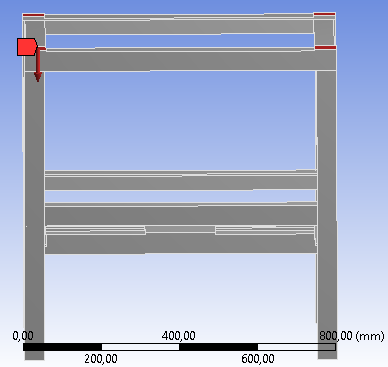
\includegraphics[scale=0.7]{figuras/an_estrutural.png}
%       \caption{Peso da chapa superior aplicada na estrutura. Fonte: Autores}
%       \label{fig:an_estrutural}
%       \end{figure}

%     A carga relacionada ao peso do motor foi aplicada na estrutura a fim de verificar a deformação máxima que este carregamento pode causar na estrutura.
%     A  Figura \ref{fig:carga_motor} ilustra a carga aplicada através da ferramenta computacional ANSYS\footnote{www.ansys.com/}.


%   \begin{figure}[H]
%       \centering
%       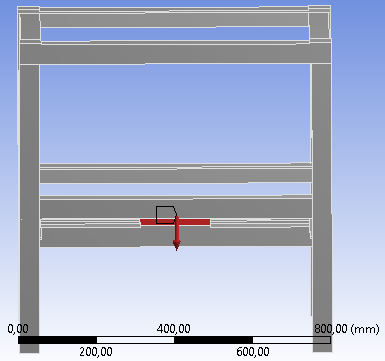
\includegraphics[scale=0.7]{figuras/carga_motor.png}
%       \caption{Peso do motor aplicado na estrutura. Fonte: Autores}
%       \label{fig:carga_motor}
%       \end{figure}

%       Com os esforços definidos, o programa computa automaticamente todos os cálculos estruturais necessários a partir das cargas aplicadas.
%       Os resultados estão mostrados na Figura \ref{fig:def_motor}.

%   \begin{figure}[H]
%       \centering
%       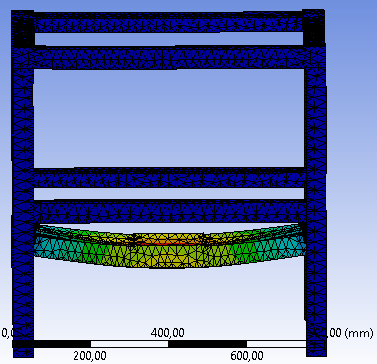
\includegraphics[scale=0.7]{figuras/def_motor.png}
%       \caption{Deformação total devido aos esforços aplicados. Fonte: Autores}
%       \label{fig:def_motor}
%       \end{figure}

%       Os resultados da simulação para deformação máxima da estrutura sob o carregamento do peso do motor são ilustrados pela Figura \ref{fig:result}.

%   \begin{figure}[H]
%       \centering
%       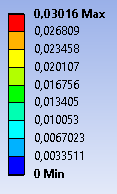
\includegraphics[scale=0.7]{figuras/result.png}
%       \caption{Resultado da deformação - Escala em mm. Fonte: Autores}
%       \label{fig:result}
%       \end{figure}

%       Pelas Figuras \ref{fig:def_motor} e \ref{fig:result}, percebe-se que o peso do motor é o responsável pela maior deformação da estrutura, mas
%       essa deformação é praticamente desprezível por ser extremamente pequena, 0,03 mm. Então a estrutura mostrou-se apta e segura para a utilização.
%     Com o intuito de ter um maior grau de segurança para validar a estrutura, diversas simulações foram feitas aumentando os valores das cargas aplicadas e as
%     deformações continuaram desprezíveis comprovando que a estrutura é válida para o projeto.

%     \vfill
% \subsubsubsection*{\textbf{Análise modal da estrutura}}

%     Uma vez que o projeto trata de uma bancada vibratória, é de suma importância analisar o comportamento da estrutura submetido a vibração. A análise modal da estrutura foi feita no software Ansys e observou-se o primeiro modo de vibração para validar a utilização da mesma.
%     A maior influência vibracional na estrutura é do motor, pelo fato do mesmo estar fixado diretamente na estrutura da mesa. A tampa superior não terá tanta relevância quanto o motor por causa das molas que amorteceram grande parte da propagação da vibração.
%     O primeiro modo de vibração da estrutura está representado na Figura \ref{fig:vib_estrutura} e corresponde a um valor de 65,83 Hz.
%     Analisando a Figura \ref{fig:vib_estrutura}, percebe-se a importância dos reforços horizontais no eixo x, pois a tendência de movimento
%     desse modo de vibração é ao longo do mesmo eixo e os reforços proporcionam uma maior rigidez para esse movimento.

%   \begin{figure}[H]
%       \centering
%       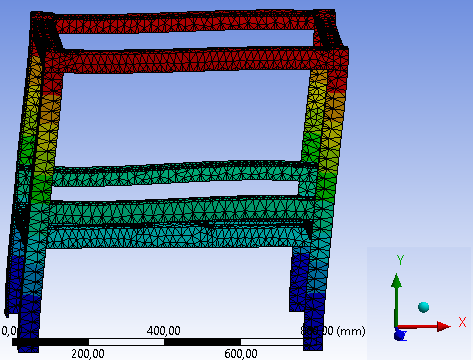
\includegraphics[scale=0.6]{figuras/vib_estrutura.png}
%       \caption{Primeiro modo de vibração da estrutura. Fonte: Autores}
%       \label{fig:vib_estrutura}
%       \end{figure}

%       Dado que o motor tem maior influência na estrutura e mesmo possui uma vibração máxima de 60 Hz e o primeiro modo de vibração foi superior
%       a esse valor, então a estrutura está validada. Para aumentar ainda mais o valor do primeiro modo de vibração, instalou-se pés vibra-stop na estrutura e,
%       assim, o grau de segurança da mesma submetida a vibração foi ampliado.

% \subsubsubsection*{\textbf{Análise modal do tampo}}

%     Tendo em vista que a rotação máxima do eixo para atender as especificações do projeto seja de 6000 rotações por minuto ou 100Hz a
%     plataforma superior da bancada não poderá ter frequência de ressonância menor que 100Hz. Para validação do mesmo foram elaborados ensaios
%     na plataforma ANSYS\footnote{www.ansys.com/} afim de verificar a frequência de ressonância do tampo.

%     A Figura \ref{fig:tampo} mostra que a frequência de ressonância do tampo é superior ao esperado(100Hz) podendo chegar até 106Hz e com isso a
%     validação da escolha deste material. A deformação máxima do tampo corresponde a 13mm.

%   \begin{figure}[H]
%       \centering
%       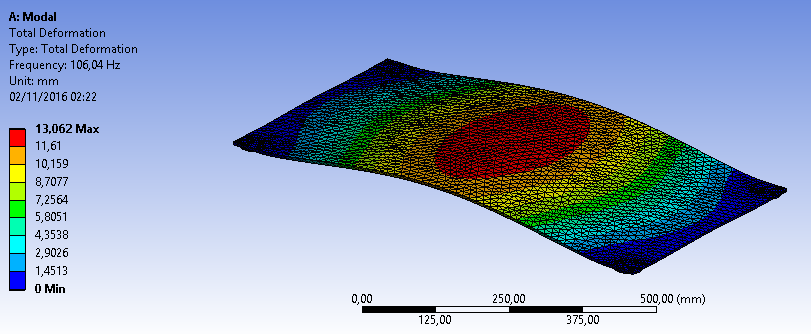
\includegraphics[scale=0.6]{figuras/tampo.png}
%       \caption{Análise modal do tampo. Fonte: Autores}
%       \label{fig:tampo}
%       \end{figure}

% \subsubsection*{\textbf{Dimensionamento das Molas}}

% Para o presente projeto foram utilizadas quatro molas de comando de válvulas de cabeçote de motor de combustão interna. A escolha desse tipo de mola se deve ao fato de possuir
% vida infinita em uso, sendo, por isso, usada nessa função pela indústria automotiva. Geralmente feitas de liga de Cromo
% e Vanádio, comandos de válvulas giram em torno de 2000 rotações por segundo por longos períodos de tempo,
% qualquer falha durante o uso terá consequências catastróficas para funcionamento do motor. A  Figura \ref{fig:mola}
% ilustra uma mola de comando de válvula utilizada em motor de automóveis.

% \begin{figure}[H]
% \centering
% 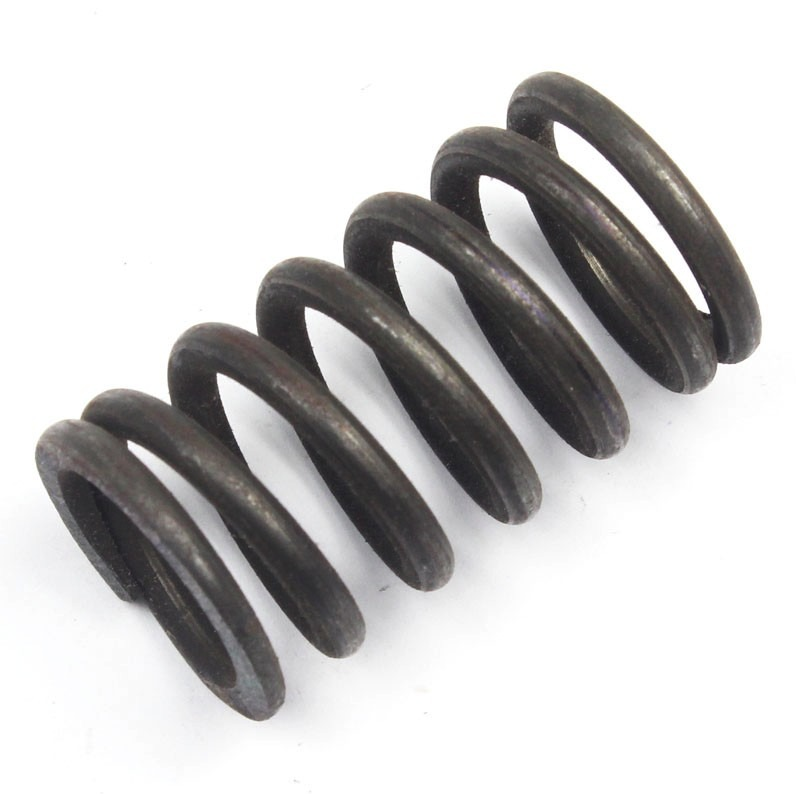
\includegraphics[scale=0.3]{figuras/mola.png}
% \caption{Mola de comando de válvula. Fonte: Mercedes Rio Diesel}
% \label{fig:mola}
% \end{figure}

% No projeto da mesa vibratória foram usadas 4 molas de comando de cabeçote uma em cada extremidade do tampo. Suas dimensões são:
% \begin{itemize}
% \item Comprimento: 45mm
% \item Diâmetro do fio da mola: 3mm
% \item Diâmetro da mola (diâmtro externo): 23,5mm
% \item Número de espiras ativas 5.
% \end{itemize}

% O uso de molas de comando de válvula, seja em um motor, seja na mesa vibratória do projeto do grupo é sempre em compressão.
% Molas de compressão possuem suas extremidades usinadas reduzindo o número de espiras ativas e contribuindo para armazenar mais energia na mola.
% Um dos principais requisitos do projeto foi a operação da mesa em uma faixa de frequência que se estende entre 70 Hz e 100Hz.
% Sabendo que um Hertz é um ciclo por segundo a máquina opera entre 70 ciclos por segundo e 100 ciclos por segundo daí constata-se que a cada ciclo dura entre:

% $$t_{min} (segundos)=\frac{1segundo}{70 ciclos/segundo}=0.0143$$
% $$t_{max} (segundos)=\frac{1segundo}{100 ciclos/segundo}=0.0100$$

% Para movimento rotativo usa-se, para cálculo de deslocamento da extremidade da mola, a expressão:

% $$deslocamento=amplitude \cos(wt)$$

% Onde t é o tempo e ômega é a velocidade angular da superfície superior da mola por tempo (todos em segundos).

% $$\omega=\frac{2\pi}{t_{ciclo}}$$

% Será usado o tempo para 100 Hz por ser o menor, mais exigente. Logo:

% $$\omega=\frac{2\pi}{t_{max}}=\frac{2\pi}{0,001s}=628,3rad/s$$

% Para encontrarmos a aceleração diferenciamos duas vezes a fórmula do deslocamento:

% $$deslocamento=amplitude * \cos(\omega t)$$
% $$aceleração=-\omega^2 * amplitude * \cos(\omega t)$$

% A aceleração máxima ocorre quando o termo $\cos(\omega t)$ equivale a 1, a situação mais extrema de operação.
% O deslocamento máximo, amplitude do movimento, foi decidido que será de 10 mm (0,01 metro). Com essa informação em mãos pode-se calcular a aceleração máxima:


% $$aceleração =628,3^2 * 0,01 *1 =3948m/s^2 $$

% Tendo em mãos o valor da aceleração é possível calcular a força que cada mola recebe. O tampo pesa exatamente 15.31 kg.
% Como as molas estão a mesma distância do centro de massa do tampo, pode-se afirmar que cada mola apoia um quarto desse valor, 3,83 kg.
% O peso máximo dos elementos que serão estudados sob a mesma são passa de 10kg e devem ser sempre apoiado no centro geométrico da mesma.
% Dessa forma cada mola suporta, devido ao corpo, no máximo, 3.33kg.

% $$ F=m*a=(3,83+3,33)kg*3948m/s^2$$
% $$ F=7,157kg*3948m/s^2$$
% $$F=28257,81kg m/s^2$$
% $$F\approx 28kN$$

% O diâmetro médio (D) de molas é dado pela equação:

% $$D=d_{ext}-d_{fio}$$
% $$D=23,5mm-3mm=20,5mm$$

% Com os valores dos dois diâmetros também é calculado o índice de mola, uma medida adimencional de curvatura da espiral da mola.

% $$C=\frac{D}{d_{fio}}$$
% $$C=\frac{20,5mm}{3mm}=6,834$$

% Econtrando o valor de \textit{Bergsträsser}

% $$K_B=\frac{4C+2}{4C-3}=\frac{4*6,834+2}{4*6,834-3}$$
% $$K_B=1,2054,$$

% Pode-se agora calcular a força limite, por segurança, para a mola atingir seu comprimento sólido. Ou seja, a força que,
% se exercida sob a mola, ocasionará contato entre suas espiras.

% $$F_s=\frac{\pi d^3 \alpha}{8 K_B D}$$ onde $$\alpha=\frac{S_{sy}}{n_s}$$

% Fs depende do material que é utilizado para confeccionar a mola, no caso de molas de comando de válvula, como informado,
% são feitas de Ligas de Cromo e Vanádio.

% Em teoria de projeto de molas a tensão última de um material pode ser encontrada por uma relação entre o seu diâmetro,
% um expoente tabelado e uma característica físicas, pela fórmula:

% $$S_{ut}=\frac{A}{d^m}$$

% Para o Cromo Vanádio tem-se, de acordo com Shigley (Projeto de Engenharia Mecânica 7ª Edição, pg 496 e 497 as características apresentadas na Tabela \ref{tab:caracteristicas_cromovanadio}.

% \begin{table}[H]
%     \begin{tabular}{|p{2cm}|p{2cm}|p{2cm}|p{2cm}|p{2cm}|p{2cm}|}
%         \hline
%         \textbf{Material} & \textbf{Número ASTM} & \textbf{Expoente} & \textbf{Diâmetro do fio (mm)} & \textbf{A (MPa $mm^{mm}$)} & \textbf{G(GPa)} \\ \hline
%         Fio de cromo-vanádio& A232& 0,168& 3&2005 &77,2                                                 \\ \hline
%     \end{tabular}
%     \caption{Características físicas do aço Cromo-Vanádio. Fonte: \cite{shigley}}
%     \label{tab:caracteristicas_cromovanadio}
% \end{table}


% Contendo assim:

% $$S_{ut}=\frac{2005}{3^{0,168}}=1667,1MPa$$

% \textit{Shigley} também afirma que, para molas de cromo-vanádio:

% $$S_{sy}=S_{ut}*0,5$$
% $$S_{sy}=1667,1*0,5=S_{sy}=833,5MPa$$

% Utilizando fator de segurança de 1,2:

% $$\alpha=\frac{833,5MPa}{1,2}=694,6MPa$$

% Retomando a fórumula:

% $$F_s=\frac{\pi d^3 \alpha}{8 K_B D} = \frac{\pi * 3mm^3 * 694,6MPa}{8*1,2054 * 20,5mm}=298,01kN$$

% Esse valor define a dimensão máxima da força que cada mola pode receber para que suas expiras se toquem. Sabendo que cada mola na mesa recebe 28kN de força, conclui-se:
% \begin{itemize}
% \item As molas suportam o limite máximo de carga sub a mesa: 10kg
% \item Sob frequencia máxima definida de 100Hz.
% \item Com fator de segurança muito alto: $n=\frac{F_S}{28kN}$
% \end{itemize}

% A rigidez (k) ou razão de mola é um parâmetro muito importante no projeto de uma mola mecânica. A teria informa que:

% $$k \frac{d^4G}{8 D^3N_a}$$

% A constante Na refere-se ao número de espiras ativas na mola, 5 e G é um valor tabelado conhecido do material da mola. No caso de fio de cromo-vanádio, G=77,2GPa

% $$k=\frac{3mm^4 77,2GPa}{8*20,5mm^3*5}=18145N/m^2$$

% Essa informação é importante para as simulações dinâmicas da mesa e tampo em softwares computacionais.  Mas é principalmente usada em considerações sobre frequência de ressonância dentro das situações de uso. Para o projeto da mesa, frequências de uso entre 70Hz e 100Hz. A fórmula a seguir apresenta, em função da razão de mola, as frequências que uma mola entra em ressonância se excitada entre placas paralelas.

% $$\omega=m\pi \sqrt{\frac{k*g}{W}}$$

% g é a aceleração da gravidade, W o peso da mola e m é o número do harmônico calculado, sendo m=1 o a frequência fundamental.

% $$W=\frac{\pi^2 d^2 D N_a \gamma}{4}$$
% $$\gamma=7,86*10^{-3}kg/mm^3$$
% $$W=17,8897N$$
% $$\omega=1\pi \sqrt{\frac{0,018145N/mm 9180mm/s^2}{17,8897}}$$

% A mola empregada na construção da mesa passa bem pelas exigências do projeto, respeitando a os requisitos de carga e frequência de utilização, já que o seu primeiro harmônico é superior ao 109 va lor máximo de 100Hz requerido pelo projeto.

% \subsubsection*{\textbf{Fixações}}

%     Tendo em vista que a problemática do projeto consiste em produzir vibrações, é de suma importância uma boa projeção das fixações que envolvem o projeto como um todo. Tais fixações devem ser atentadas para que não haja falhas ou até mesmo perda de funcionalidade de componentes. Nos tópicos seguintes são discutidas como serão as fixações bem como suas respectivas justificativas.

% \subsubsubsection*{\textbf{Fixação dos pés}}

%     Os pés de borracha que sustentam a estrutura do projeto consistem em fixação por parafuso e porca. Para que esta fixação não comprometa a integridade da estrutura, foram elaborados apoios com furação iguais aos das roscas dos pés, as quais são de meia polegada. Além disso, como o projeto consiste em constantes vibrações sobre a estrutura, foram realizados travamento para que as porcas não venham folgar ou até mesmo soltar ao longo do tempo.
%     Tendo em vista este problema a fixação é feita por duas porcas na parte superior da estrutura, como podemos ver na Figura \ref{fig:config_pes}. A fim de ajustar erros de construção obtidos pela solda da estrutura a qual provocou desnível na mesma foram colocadas arruelas na medida certa até que houvesse o nivelamento da estrutura.

%     \begin{figure}[H]
%       \centering
%       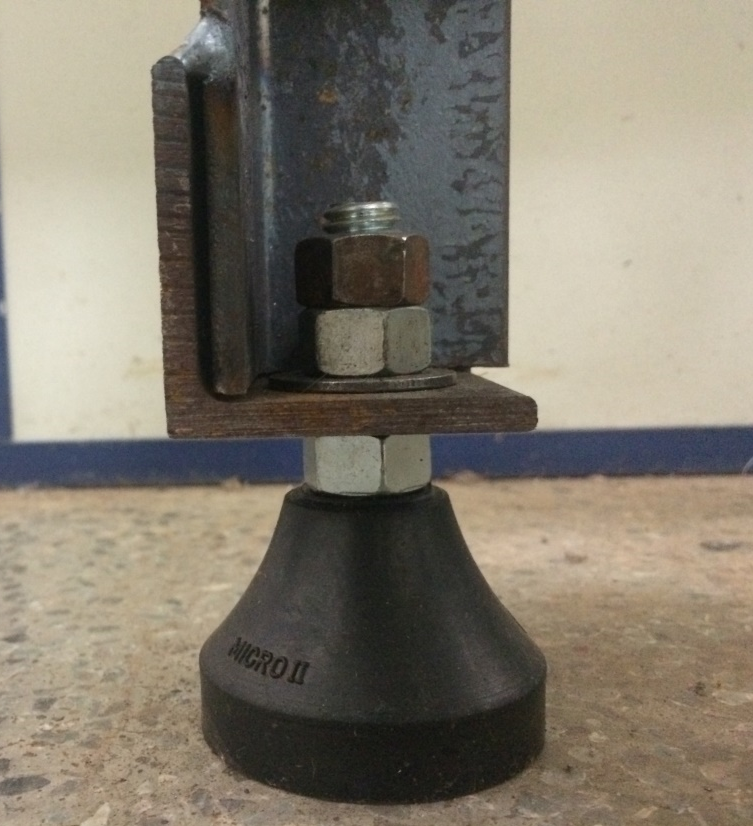
\includegraphics[scale=0.4]{figuras/config_pes_jpg.png}
%       \caption{Configuração da fixação dos pés. Fonte: Autores}
%       \label{fig:config_pes}
%       \end{figure}

% \subsubsubsection*{\textbf{Fixação do motor}}

%     O motor de indução trifásico do tipo gaiola o qual poderá exercer frequências de até 60Hz sobre a estrutura é fixado a partir de parafusos, arruelas de pressão e porcas. Como a constância de vibração do motor exercido sobre a estrutura é alta a necessidade de colocar coxins entre a carcaça do motor e a estrutura foi um ponto crucial para o projeto, absorvendo assim as vibrações do motor para com a estrutura. Para que as porcas não venham a folgar ou até mesmo soltar durante o funcionamento do motor foram colocadas arruelas de pressão, garantindo assim com que o conjunto parafuso e porca fique fixo e não se soltem a longo prazo.

% \subsubsubsection*{\textbf{Fixação das molas}}

%     As molas são os componentes mais delicados do projeto, tendo em vista que será o componente que mais sofrerá esforço. Com base nisto é de suma importância estar atento a todos os detalhes deste item do projeto. Para que não haja falha das molas, é de entendimento que tais componentes não podem ser soldados na estrutura, para que o projeto atenda tais requisitos as molas são fixadas na estrutura através de interferência do diâmetro interno da mola para com copinhos de fixação que foram projetados pelos próprios autores. Para que não houvesse solda entre os copinhos com a estrutura foram elaboradas chapas de sustentação dos copinhos, nos quais tem furação para que a solda fosse elaborada por baixo dos copinhos.
%     Para melhor entendimento a Figura \ref{fig:config_copinhos} ilustra a configuração dos copinhos.

% \begin{figure}[H]
% \centering
% 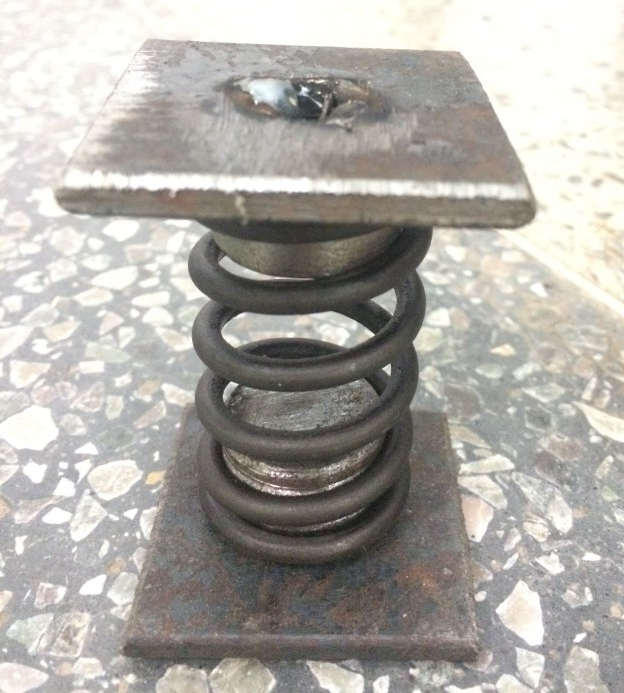
\includegraphics[scale=0.5]{figuras/config_copinhos.png}
% \caption{Configuração das molas. Fonte: Autores}
% \label{fig:config_copinhos}
% \end{figure}

% \subsubsection*{\textbf{Sistema de Transmissão}}

% \subsubsubsection*{\textbf{Polias e correias}}

%     As polias são peças cilíndricas, movimentadas pela rotação do eixo do motor e pelas correias. Os tipos de polia são determinados pela forma da superfície na qual a correia se assenta. Correias são elementos de máquinas que transmitem movimento de rotação entre dois eixos (motor e movido) por intermédio de polias. Elas são empregadas quando se pretende transmitir potência de um veio para o outro a uma distância em que o uso de engrenagens é inviável. Para o sistema em questão será usada as polias do tipo Trapezoidal ou V múltipla.

%     A correia em V ou trapezoidal é inteiriça, fabricada com seção transversal em forma de trapézio. É feita de borracha revestida de lona e é formada no seu interior por cordonéis vulcanizados para suportar as forças de tração. O emprego da correia trapezoidal ou em V é preferível ao da correia plana pelos seguintes motivos: Praticamente não apresenta deslizamento; Permite o uso de polias bem próximas; Elimina os ruídos e os choques, típicos das correias emendadas (planas).

%     Como as correias têm características diferentes de fabricante para fabricante, é aconselhável seguir as instruções que eles forneçam. A partir destes elementos pretende-se selecionar a polia do tipo guia com correia do tipo trapezoidal a ser usada observando o tipo, a secção e o comprimento primitivo, potência a ser transmitida, tipos de máquina motoras e movidas, velocidade angular da polia motora e da polia movida, distância entre os eixos da polia motora e da polia movida, distância entre os eixos das polias, na qual o comprimento máximo admitido deve ser igual a três o produto da soma dos diâmetros da polia motora e movida e finalmente o tipo de carga(uniforme, choques moderados, choques intensos).

%     A polia maior acoplada na saída do eixo do motor tem diâmetro de 250mm, feita de alumínio fundido e é fixada na ponta de eixo do motor através de chavetas e parafusos. A Figura\ref{fig:config_polia} ilustra o esboço do acoplamento do motor com a polia e da polia com a correia.

% \vfill

% \begin{figure}[H]
% \centering
% 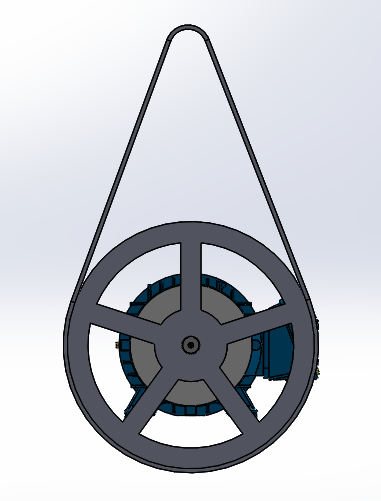
\includegraphics[scale=0.6]{figuras/config_polia.png}
% \caption{Configuração do acoplamento polia, motor e correia. Fonte: Autores}
% \label{fig:config_polia}
% \end{figure}

% \subsubsubsection*{\textbf{Mancal e eixo}}

%     Fora escolhido como mecanismo de transmissão de movimento deste projeto, mancal e eixo centralizado. Mancal é um componente de uma máquina que possui a função de permitir com que o eixo flutue em uma posição determinada, ou seja, funciona como um suporte ou guia a fim de que o eixo possa ser utilizado sem perdas de desempenho devido ao contato com peças externas.

%     A escolha do mancal deve-se ao fato de suas diversas vantagens que se enquadram nos pré-requisitos do projeto tais como: amortecem as vibrações, choques e ruídos, construção simples e custos menores nos projetos dependendo da utilização e finalidade. Os mancais podem ser separados em dois grupos: os de rolamento e os de deslizamento. O que fora escolhido no projeto foi o mancal de deslizamento devido ao fato dele adaptarem-se facilmente as circunstâncias, simples de montar e desmontar e de já o possuirmos.

%     Ao se escolher os mancais de deslizamento houve a preocupação de tomar alguns cuidados em relação a sua manutenção, esses são sujeitos as forças de atrito estas por sua vez surgem devido a rotação do eixo que exercerá carga nos apoios, ou seja, deve-se haver um sistema de lubrificação com o intuito de minimizar as perdas pelo atrito

%     Os mancais de deslizamentos são constituídos de bucha (corpo cilíndrico oco que envolve o eixo) fixada num suporte, estes mancais são utilizados em máquinas pesadas ou em equipamentos com pouca rotação, pois devido ao atrito os componentes aquecem. Ao se utilizar a bucha e lubrificantes reduzimos o atrito e melhoramos a rotação e consequentemente melhoramos o desempenho da rotação.

%     O objetivo em se utilizar este sistema é colocar uma massa desbalanceada com o intuito de que gere na mesa as vibrações desejadas, para que isso ocorre tem que levar em consideração tais observações: Massa desbalanceadora, que se trata de um peso com uma distribuição não uniforme por meio deste podemos obter amplitudes de vibração ou seja quanto maior for a massa desbalanceada maior será a amplitude de vibração; Raio da ação da massa desbalanceadora, pois quanto maior for o raio desta massa maior será a amplitude para a mesma massa desbalanceada; Rotação da polia, em relação a esta podemos analisar que ao se aumentar a rotação aumenta-se a amplitude de vibração de acordo com o desbalanceamento. A Figura \ref{fig:mancal} ilustra melhor o mancal e seu respectivo eixo a ser utilizado no projeto.

% \begin{figure}[H]
% \centering
% 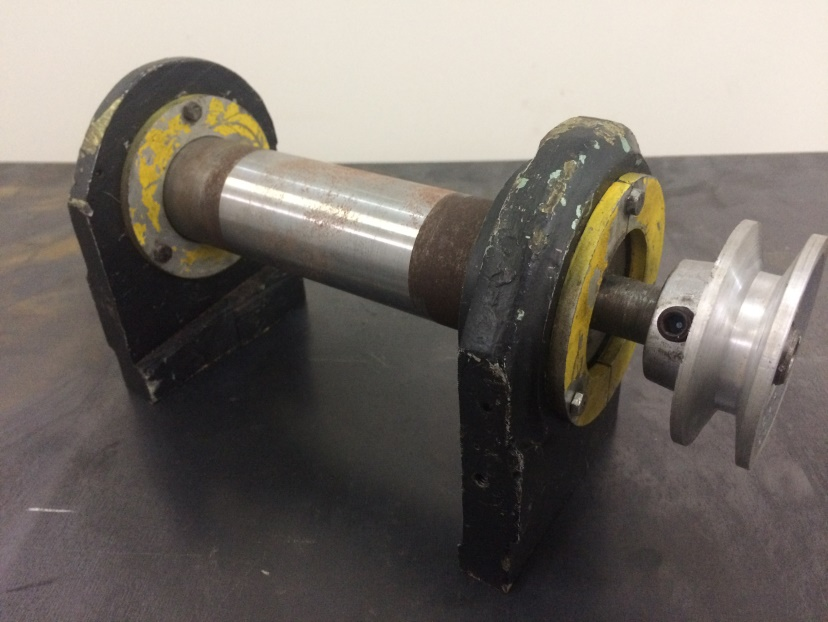
\includegraphics[scale=0.9]{figuras/mancal.jpg}
% \caption{Mancal a ser utilizado com seu respectivo eixo e polia acoplados. Fonte: Autores}
% \label{fig:mancal}
% \end{figure}

% \subsubsubsection{\textbf{Relação polia/eixo}}

%     Tendo em vista que a rotação máxima do motor é de 1720 rotações por minuto e que esta rotação equivale apenas a 28,67Hz. Como uma das primícias do projeto visa chegar à vibrações de até 100Hz é necessário aumentar a rotação do motor. Para tal utilizamos uma relação entre polias para que seja possível chegar uma rotação de no mínimo 6000 rotações por minuto o que equivale a uma relação de 3,5. Tendo em vista a polia maior com diâmetro de 250mm é necessário que a polia menor seja de diâmetro máximo de 71,42mm. Entre as polias comerciais a menor mais próxima do valor citado anteriormente equivale a um diâmetro de 60mm atendendo assim as especificações do projeto, podendo assim o eixo fixado na mesa chegar até 7166 rotações por minuto.


\section{Projeto Eletromecânico}

\label{desenvolvimento_eletromecanica}

Máquina elétrica é um dispositivo capaz de transformar energia mecânica em elétrica ou vice-versa. Quando a máquina converte energia elétrica em energia mecânica ela trabalha como um motor e quando transforma energia mecânica em elétrica ela trabalha como um gerador, sendo assim, toda máquina elétrica pode funcionar dos dois jeitos, tanto como gerador como motor. \cite{chapman}  \\

No projeto em questão, será usado motores de indução trifásicos com o intuito de acionar um sistema com objetos desbalanceados presos em uma bancada, gerando assim uma vibração nesta bancada. Para realizar esta vibração, a velocidade do motor será alterada com o uso de um inversor de frequência. O conjunto motor+inversor dimensionado deverá atender o torque solicitado e as velocidades solicitadas por todo o sistema.\\
\\
\textbf{MOTOR DE INDUÇÃO TRIFÁSICO}\\

Os motores de indução trifásicos ou monofásicos são os mais amplamente usados em acionamentos elétricos, pois sua eficiência é alta, em torno de 85\%.\cite{WEG}
\\

\textbf{Princípio de funcionamento do motor de indução}: quando se aplica uma tensão trifásica no estator, gera-se um conjunto de correntes trifásicas circulando no estator. Um campo magnético girante então é produzido e este campo passa pelas barras do rotor e induz tensão nelas. Como existem dois campos magnéticos, um no estator e um no rotor, aparecerá uma força entre o rotor e o estator que fará com que o rotor gire, pois este está solto e seu eixo montado em rolamentos, gerando assim torque no seu eixo \cite{chapman}. A velocidade de rotação do campo magnético é dada por:


    \begin{equation}\label{Rotação de Campo Mag.}
            Nsinc=(120*f)/P
    \end{equation}

onde f é a frequência do sistema de alimentação em hertz e P é o número de polos da máquina. \cite{chapman}
\\

O rotor não gira na velocidade síncrona, pois se isso acontecesse o rotor estaria estacionário em relação ao campo magnético, logo, não haveria tensão induzida e consequentemente não haveria corrente nem campo magnético no rotor. Sem campo magnético no rotor o torque induzido seria zero e o motor perderia velocidade por causa do atrito. Portanto, um MIT pode ganhar velocidade até próximo da velocidade síncrona, mas nunca alcança-la exatamente.\cite{chapman}
\\

A diferença entre a velocidade síncrona e a velocidade do rotor, chama-se velocidade de escorregamento (Nesc). \cite{chapman}

    \begin{equation}\label{Velocidade de Escorregamento .}
            Nesc=Nsinc-Nm
    \end{equation}
    

Segundo \cite{chapman} outro termo usado, é o chamado escorregamento (S), que é a velocidade relativa expressa em uma base por porcentagem.
  
  
  \begin{equation}\label{Escorregamento S}
           S=(Nesc/Nsinc) x 100\%
    \end{equation}

A velocidade mecânica do rotor pode ser expressa em função do escorregamento e da velocidade síncrona, logo:


  \begin{equation}\label{Velocidade Mecânica do Rotor}
         Nm=(1-S)Nsinc
    \end{equation}

O tipo de máquina de indução polifásica mais comumente usada é o rotor de gaiola de esquilo \ref{fig:motor}, no qual barras condutoras encaixadas em ranhuras no ferro do rotor e curto-circuitadas em cada lado por anéis condutores caracterizam seu enrolamento. \cite{Fitzgerald}

\begin{figure}[!ht]
\centering
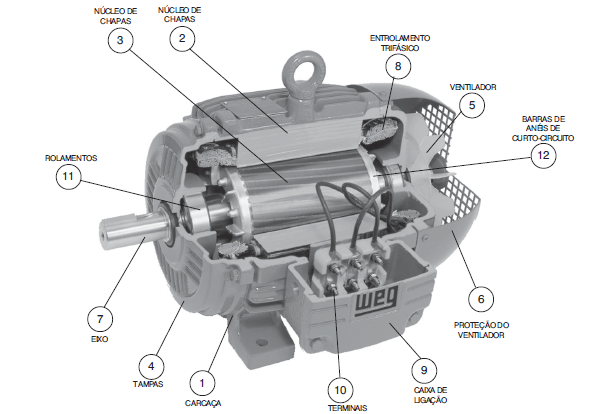
\includegraphics[keepaspectratio=true,scale=0.8]{figuras/motor.png}
\caption{Motor gaiola de esquilo. Fonte:\cite{WEG}}
\label{fig:motor}

\end{figure}

\textbf{CURVAS CARACTERÍSTICAS DO MOTOR DE INDUÇÃO}\\

A curva de torque x velocidade mostra a relação entre o torque desenvolvido pelo motor e sua rotação. Na partida o torque será de aproximadamente 2 a 2,5 vezes o torque nominal. De acordo com o aumento da velocidade este vai diminuindo até atingir valores de 1,5 a 1,7 do torque nominal.\cite{WEG} A medida que essa velocidade aumenta o torque vai aumentando novamente até atingir seu valor de pico máximo e depois vai diminuindo até chegar no seu 
valor nominal, como mostra a Figura \ref{fig:curvas_motor}.
% valor nominal, como mostra a figura abaixo:

\begin{figure}[!ht]
\centering
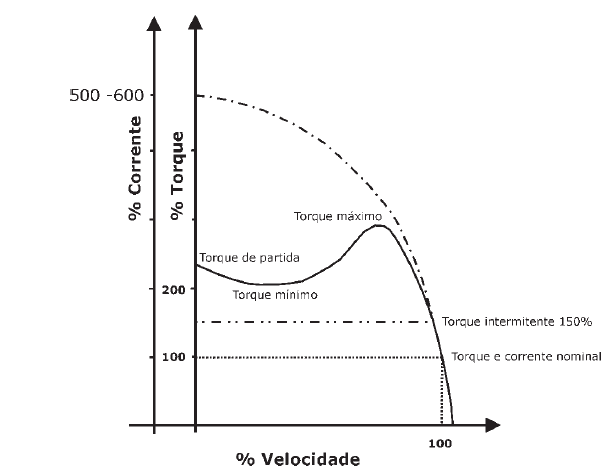
\includegraphics[scale=0.8]{figuras/grafico_motor.png}
\caption{Curvas Torque x Velocidade e Corrente x Velocidade para MI de rotor gaiola de esquilo. Fonte:\cite{WEG}}
\label{fig:curvas_motor}
\end{figure}

A curva de Corrente x Velocidade mostra a relação entre a corrente consumida pelo motor em função da velocidade. Como pode-se observar na Figura \ref{fig:curvas_motor}, quando o motor é acionado tem-se um pico de corrente de 5 a 6 vezes maior que a corrente nominal, diminuindo à medida que a velocidade aumenta até atingir um valor permanente de funcionamento.\\

\text Esses picos de corrente causado pelo acionamento de motores não é bom para a rede elétrica e para os demais aparelhos, por isso, existe maneiras de partidas mais suaves como a partida estrela-triângulo (tem o valor da corrente diminuído cerca de 1/3 da corrente de partida) e a soft-starter que é com o uso de um inversor de frequência como será explicado logo a frente.\\

\textbf{ESPECIFICAÇÕES DO MOTOR ANÁLISE DO MOTOR}\\
O Motor Trifásico IP55 pode ser aplicado em bombas, ventiladores, exaustores, britadores, moinhos, talhas, compressores e outras aplicações que requeiram motores assíncronos de indução trifásicos. Pode ser utilizado, ainda, com inversores em tensões menores que 575V. (WEG)\\

O Motor Trifásico IP55 pode ser aplicado em bombas, ventiladores, exaustores, britadores, moinhos, talhas, compressores e outras aplicações que requeiram motores assíncronos de indução trifásicos. Pode ser utilizado, ainda, com inversores em tensões menores que 575V.\\

Se ligarmos os três sistemas monofásicos entre si, como indicam as figuras \ref{fig:TRIANGULO}, podemos eliminar três fios, deixando apenas um em cada ponto de ligação, e o sistema trifásico ficará reduzido a três fios L1, L2 e L3.Tensão de linha ( U ) É a tensão nominal do sistema trifásico aplicada entre dois quaisquer dos
três fios L1, L2 e L3.

\begin{figure}[!ht]
\centering
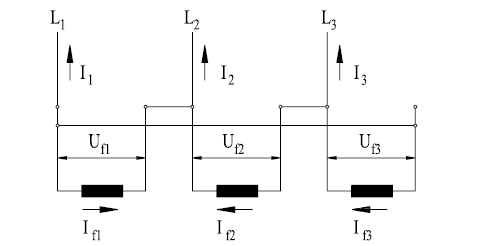
\includegraphics[scale=0.8]{figuras/TRIANGULO.png}
\caption{Ligação em Delta (triângulo)}
\label{fig:TRIANGULO}
\end{figure}

Ligando um dos fios de cada sistema monofásico a um ponto comum aos três, os três fios restantes formam um sistema trifásico em estrela \ref{fig:ESTRELA}. Às vezes, o sistema trifásico em estrela é “a quatro fios” ou “com neutro”. O quarto fio é ligado ao ponto comum às três fases. A tensão de linha ou tensão nominal do sistema trifásico e a corrente de linha, são definidas do mesmo modo que na ligação triângulo.

De acordo com o abordado acima, a ligação do motor será em estrela, dado que a disponibilidade de tensão é 220V na rede elétrica local.

\begin{figure}[!ht]
\centering
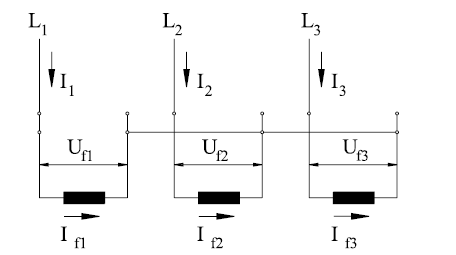
\includegraphics[scale=0.8]{figuras/ESTRELA.png}
\caption{Ligação em estrela}
\label{fig:ESTRELA}
\end{figure}

Conforme as suas características de conjugado em relação à velocidade e corrente de partida, os motores de indução trifásicos com rotor de gaiola, são classificados em categorias, cada uma adequada a um tipo de carga. Estas categorias são definidas em norma (NBR 7094), e são as seguintes: N, H e D. 

Para o tipo de motor avaliado temos que a categoria de conjugado é do tipo N. (weg)

\textbf{Categoria N:} Conjugado de partida normal, corrente de partida normal; baixo escorregamento.(weg)

Na \ref{} verifica-se como se comportam as três principais categorias de motores de indução de gaiola em função da velocidade.

\begin{figure}[!ht]
\centering
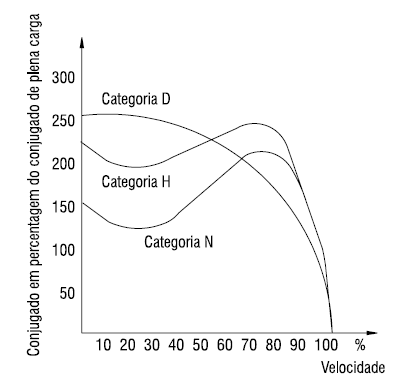
\includegraphics[scale=0.8]{figuras/conjugado_N.png}
\caption{Curvas Conjugado X Velocidade das diferentes categorias}
\label{fig:conjugado_N}
\end{figure}

%TABELAA DOS DADOS DO MOTOR

\begin{figure}[!ht]
\centering
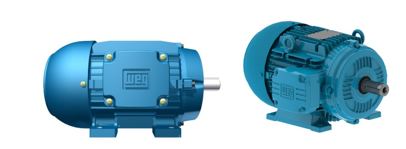
\includegraphics[scale=0.8]{figuras/motorgaiola.png}
\caption{Motor de indução trifásico do tipo gaiola}
\label{fig:motorgaiola}
\end{figure}

\begin{figure}[!ht]
\centering
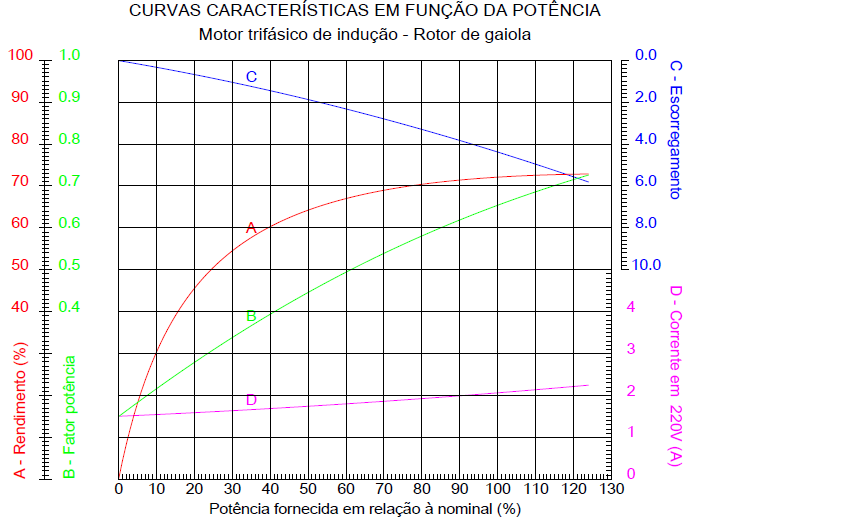
\includegraphics[scale=0.8]{figuras/Motor_potencia.png}
\caption{Curvas características em função da potência Fonte:(weg)}
\label{fig:motor_potencia}
\end{figure}

\begin{figure}[!ht]
\centering
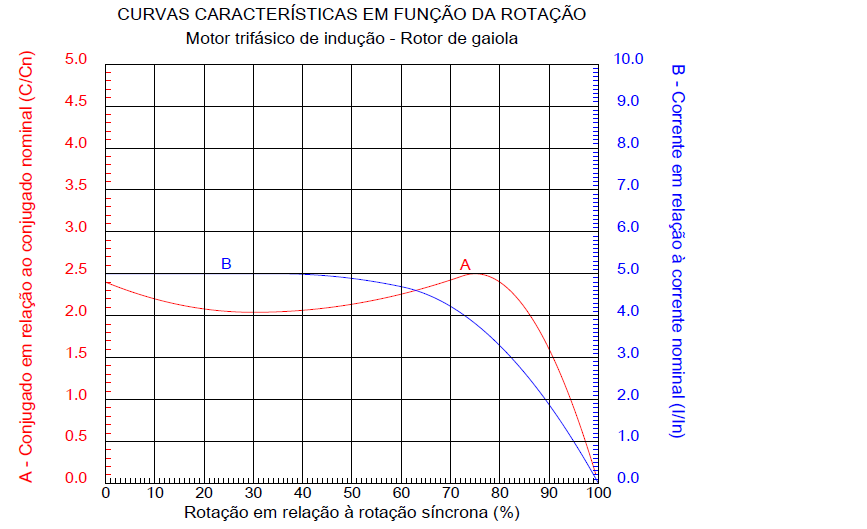
\includegraphics[scale=0.8]{figuras/motor_rota__o.png}
\caption{Curvas características em função da potência Fonte:(weg)}
\label{fig:motor_rota__o}
\end{figure}

Como já mencionado algumas vezes neste trabalho, uma das principais preocupações que devemos ter em relação aos motores elétricos é sua temperatura de operação, cada motor possui um tipo de classe de isolamento que nada mais é que um tipo diferente de isolante em seus enrolamentos (ou a quantidade dele), esses isolantes servem, como o próprio nome diz, para isolar os fios um dos outros das bobinas, no caso dos motores gaiola, da bobina do estator.


\begin{figure}[!ht]
\centering
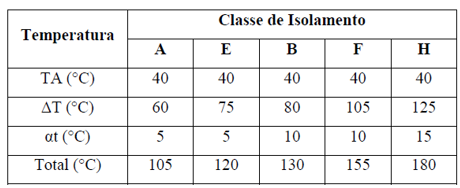
\includegraphics[scale=0.8]{figuras/tabela_isolamento.png}
\label{fig:tabela_isolamento}
\end{figure}


\textbf{INVERSORES DE FREQUÊNCIA}\\

A tensão de rede de frequência constante é transformada em uma tensão com frequência e amplitude variáveis pelo inversor,     assim ocorre uma variação na velocidade do campo girante. O inversor de frequência é vantajoso para as indústrias, porque o controle é à distância (comunicação serial), há redução de custos (corrente de partida limitada), produtividade aumentada (velocidade de operação devidamente adequada ao processo), eficiência energética (rendimento superior a 97\%) e agilidade para os sistemas de posicionamento (partidas e frenagens acontecem em milésimos de segundos) \cite{WEG2}.
    Analisando as equações:
    
    \begin{equation}\label{Rotação Sinc.}
            Nsinc=(120*f)/P
    \end{equation}
    e
    \begin{equation}\label{Rotação Sinc.}
     Nm=(1-S)Nsinc
    \end{equation} 
    
     verifica-se que a variação do escorregamento é capaz de modificar a velocidade de rotação de um motor de indução trifásico; o número de polos do motor ou da frequência da tensão no estator também modificam essa velocidade. O método mais eficaz para a variação da velocidade de rotação de motor de indução tem sido a utilização de inversor de frequência. \cite{WEG2}.  
     
     \textbf PARTIDA E FRENAGEM DE MIT (MOTOR DE INDUÇÃO TRIFÁSICO) COM INVERSOR DE FREQUÊNCIA\\
     
     O inversor de frequência trabalha com rampas para partida e frenagem. Na partida é utilizada a rampa de aceleração, a velocidade inicia em zero e atinge a velocidade desejada, podendo ajudar o tempo numa faixa de milésimos de segundo. 
    A frequência do rotor é maior do que a frequência do estator durante a frenagem, dessa forma é provocado um fluxo reverso da energia do rotor diretamente ao estator \cite{covino}. A rampa de desaceleração é responsável por controlar a frenagem, esse processo se dá pela redução de forma controlada da frequência aplicada ao motor.
    A figura abaixo evidencia as rampas de aceleração e desaceleração:\\

 \begin{figure}[h]    
 		\centering
		\label{oldr}
		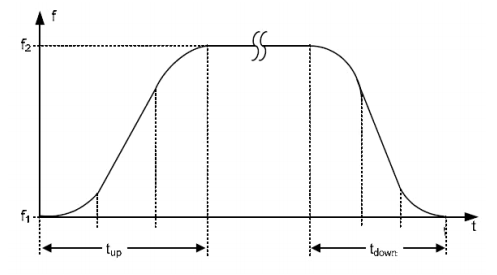
\includegraphics[keepaspectratio=true,scale=0.75]{figuras/rampa_aceleracao.png}
		\caption{Rampas de aceleração e desaceleração geradas pelo inversor de frequência \cite{siemens}.}
		\end{figure}  
        
        
        O projeto contará especificamente com o inversor Power Flex 40 de 0,5CV a 380V da consagrada marca Allen Bradley, com vasta tradição de aplicabilidade na indústria. 
        
        %Botar a foto inversor_final que está no drive aqui
        
        A principal vantagem 
        
        
\textbf APLICABILIDADE AO SISTEMA DA MESA DE VIBRAÇÃO\\

O inversor assume papel vital, pois uma vez que é responsável por interfacear o mecanismo de potência e controle para com a aplicação desejada, no projeto será quem, de fato, condicionará o motor a operar segundo as especificações retornadas do sistema de controle. As rotinas de testes da bancada entregam ao inversor de forma instantânea os dados de frequência de operação, e consequentemente de velocidade a qual a mesa responte com a vibração esperada. 

Os parâmetros de entrada do inversor são entregues segundo o consagrado protocolo de comunicação industrial MODBUS, que se trata de uma estrutura de mensagem aberta, amplamente utilizado em razão da sua simplicidade e facilidade de implementação.\\

\textbf DIMENSIONAMENTO DE CABOS\\

Dada as cargas de maior relevância do presente projeto, inversores, um par de motores e os circuitos eletrônicos do sistema, será realizado um levantamento de carga de projeto de forma a permitir com boa aproximação a obtenção dos parâmetros dos condutores de alimentação de potencia do circuito principal e dos sub-circuitos.

    O sistema motor é constituído por uma unidade de motor WEG 0,5CV 220/380V, 1720RPM os qual apresenta, segundo o fabricante, corrente nominal de 2,07A configuração estrela (380V) totalizando 0,58A por fase.
    
    O Inversor, Allen Breadley 0,5Cv 380V, designados para o controle de acionamento e velocidade de rotação do projeto, apresentam para tal, um autoconsumo de aproximadamente 50W, contribuindo com uma corrente de 0,13A.
    
    As cargas secundárias constituídas pelos sistemas de monitoramento e controle acoplados ao sistema não devem  ser menosprezadas, no entanto para fins de dimensionamento, será considerada a alimentação por uma fonte retificadora DC com entrega máxima de 2A.
    
    A tabela abaixo representa um compilado dos dados de corrente do projeto e os respectivos resultados dos dimensionamentos de secção mínimos segundo a normatização vigente (NBR 5410, NBR6818 e EB98 ABNT).
    
    \begin{table}[h]
	\centering
	\label{tab01}
	
	\begin{tabular}{llllll}
		\toprule
		\textbf{Item} & \textbf{Qtd} & 
        \textbf{Potência} & \textbf{Corrente Tot.}  & \textbf{Corrente/f}  & 
        \textbf{Secção/F NBR 6418} \\
		\midrule
		Motor & 1 & 370W & 2,07A & 0,58A & 2,5mm2 \\
		Inversor & 1 & 50W & 0,13A & 0,07 & 2,5mm2 \\
		Circ. COntrole & 1 & 24W & 2A & 2A(Fase 1) & 2,5mm2 \\
		\bottomrule
	\end{tabular}

	\caption{Correntes dos Sub-circuitos}
\end{table}

Dessa forma, levando em consideração as correntes totais por fase do sistema, chegamos aos presentes resultados para as correntes totais nos barramentos de acesso:

    \begin{table}[h]
	\centering
	\label{tab01}
	
	\begin{tabular}{llll}
		\toprule
		\textbf{Circuito} & \textbf{Fase 1} & \textbf{Fase 2} & \textbf{Fase 3}\\
		\midrule
		Motor e Inversor & 0,65A & 0,65A & 0,65A \\
		Controle & 2,00A & 0A & 0A \\
        Acesso de Energia & 2,65A & 0,65A & 0,65A \\
		\bottomrule
	\end{tabular}

	\caption{Correntes no Acesso de Força}
\end{table}

Dessa forma, ficando válido a bitola mínima estabelecida pela norma NBR5410 de 2,5mm para circuitos de força em todos os estágios sejam de acesso ou interconexões. \cite{NBR5410}

No que tange o dimensionamento do condutor neutro, é de boa prática que seja dimensionado segundo os mesmos parâmetros dos condutores de fase, motivado, principalmente pela carga harmônica injetada pelos circuitos não lineares dos inversores, que podem induzir a circulação de carga no condutor neutro.

    E finalmente, em relação ao condutor terra, esse deve ser capaz de atender aos requisitos mínimos de corrente de falta possivelmente possa ocorrer. Para tal, a recomendação dos fabricantes é que se utilize, no mínimo, o mesmo diâmetro dos alimentadores.

    
    


     







\section{Projeto Eletroeletrônico}

\label{desenvolvimento_eletroeletronica}

Nesta seção é descrito o detalhamento da solução do módulo de eletroeletrônica, resultante das duas primeiras fases,
e o seu projeto e construção, resultante da Fase 03.

\subsection{Detalhamento de Solução}

\subsubsection*{Desenvolvimento de arquitetura para o sistema de sensoriamento}

A arquitetura do projeto da mesa deve cumprir os seguintes pré-requisitos:

\begin{itemize}
    \item Ser escalável, isto é, comportar um aumento de sensores disponíveis. Para isso, optou-se por sensores interfaceados por I2C, e um sistema baseado em multiplexadores e Registradores de deslocamento para o controle da leitura do sensor.
    \item Garantir a correta frequencia de amostragem para os sensores disponibilizados.
    \item Possuir interface de comunicação externa com qualquer dispositivo que queira controlar parametros de vibração da mesa, como a frequencia.
    \item Possuir a função de “módulo mestre”, controlando todos os demais, e sendo controlado via UART.
\end{itemize}

\subsubsection*{Desenvolvimento de arquitetura para um sistema de controle de motores}

A arquitetura do projeto do módulo de controle de motores deve cumprir os seguintes pré-requisitos:

\begin{itemize}
    \item Ser  controlável via I2C, recebendo e enviando comandos do módulo mestre.
    \item Possuir capacidade de controle em malha fechada da frequencia da mesa.
    \item Possuir capacidade de controle do motor.
\end{itemize}

\subsection{Projeto e construção}

Um módulo BSP é uma coletânia de códigos básicos de microcontrolador, que implementam um a um todas as suas funcionalidades. Dessa forma, funções mais alto nível são disponibilizadas para a aplicação, tornando-a mais genérica e permitindo que a mesma possa suportar mais de um microcontrolador ao mesmo tempo. \\
Para o projeto em questão, as seguintes implementações específicas de MSP430 foram criadas. Todas são suportadas para dois microntoladores (MSP430F2274 e MSP430G25543), de forma que se reduz ao mínimo o tempo de desenvolvimento de código, sem perder a robustez e flexibilidade.

\begin{figure}[htbp]
    \centering
        \includegraphics[scale=0.6]{figuras/bsp.png}
    \caption{Pacotes implementados para o BSP}
    \label{bsp-scheme}
\end{figure}

\subsection*{Sistema Bevim}

O sistema BeVim é composto pelos seguintes módulos:

\begin{itemize}
    \item Módulo de Sensoriamento - Parte responsável pela leitura de sensores, comunicação com a CPU e controle dos módulos de motores.
    \item Módulo de Motor - Parte responsável pelo controle de inversores, e pela retroalimentação em malha fechada para atingir frequencias altas.
\end{itemize}

Ambos os moódulos são conectados entre si por uma rede I2C (InterIntegrated Circuits), onde o módulo de sensoriamento sempre atua como mestre no processo de comunicação. Esse procedimento foi escolhido pela possibilidade de se adicionar de maneira fácil outros módulos (de motor, por exemplo, ou outros que sejam de interesse a serem desenvolvidos), não interferindo com outros sistemas perifericos a mesa.

\subsubsection*{Módulo de Sensoriamento}
O módulo de sensoriamento é o responsável pela implementação da interface (via protocolo BeVim) com o sistema que controla a mesa em alto nível - a CPU. Ao mesmo tempo, esse módulo executa um controle da leitura dos sensores digitais do projeto, e dos outros módulos acoplados (os de motores).

\begin{figure}[htbp]
    \centering
        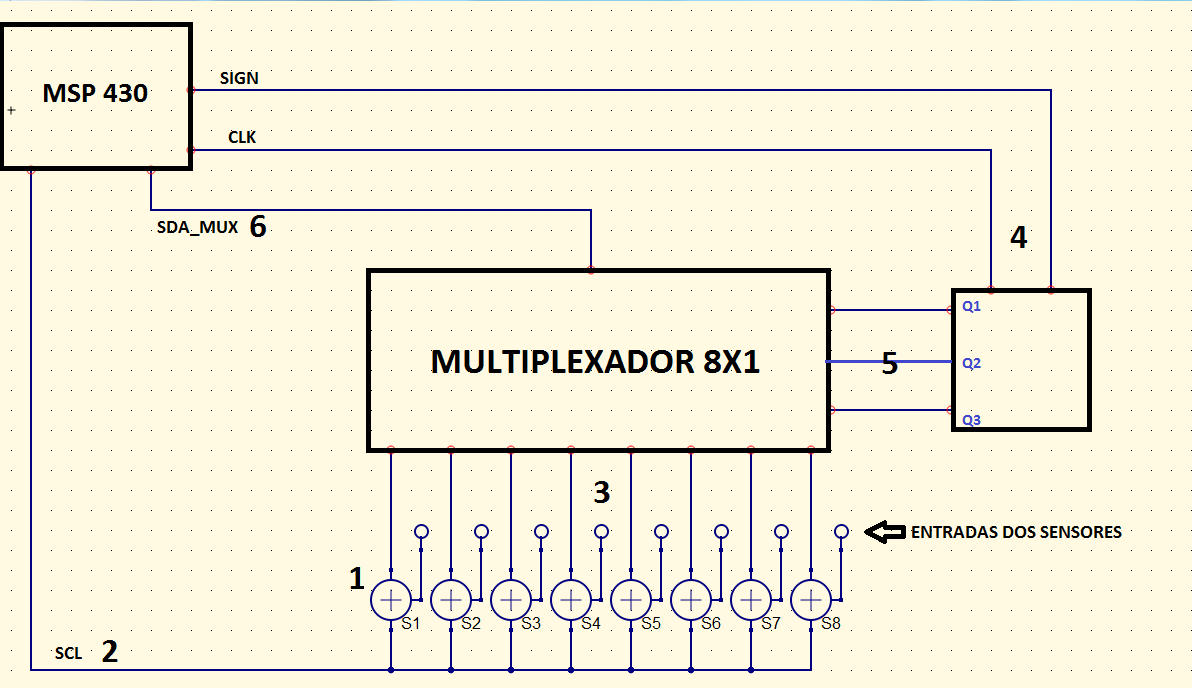
\includegraphics[scale=0.6]{figuras/mod_sensor.png}
    \caption{Módulo de Sensoriamento}
    \label{mod_sensor}
\end{figure}

Itens da Figura \ref{mod_sensor}:

\begin{enumerate}
    \item Conectores DB9, que receptam os sinais dos acelerômetros.
    \item Os sensores recebem sinais de clock provindos do microcontrolador, através do sinal SCL da rede I2C.
    \item Os sinais de dados de cada sensor servem como entrada de um multiplexador 8x1.
    \item O MSP430, através de duas portas GPIO's, controlam um registrador responsável pelas portas seletoras do multiplexador. Uma porta é o sinal serial de seleção “sign” e a outra é o clock “clk”.
    \item O conjunto do registrador com o multiplexador é capaz de selecionar qual sensor será aferido pelo sistema.
    \item O dado do sensor selecionado é enviado para a rede I2C através do caminho SDA-MUX
\end{enumerate}

\subsubsection*{Módulo de Motor}

\begin{figure}[htbp]
    \centering
        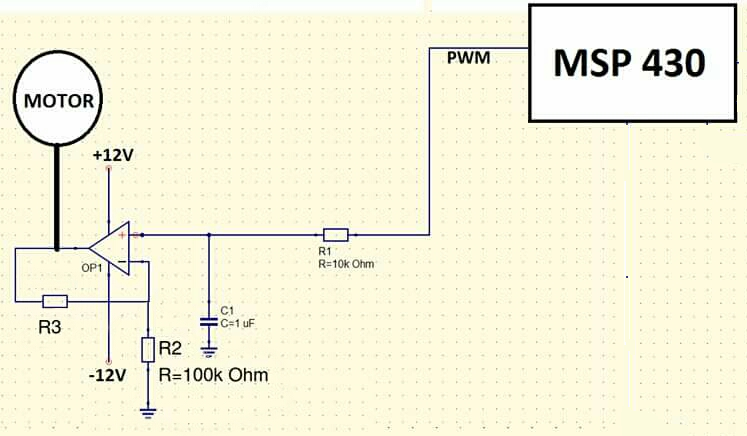
\includegraphics[scale=0.6]{figuras/mod_motor.png}
    \caption{Módulo do Motor}
    \label{mod_motor}
\end{figure}


\subsection*{Circuito Completo}

\begin{figure}[htbp]
    \centering
        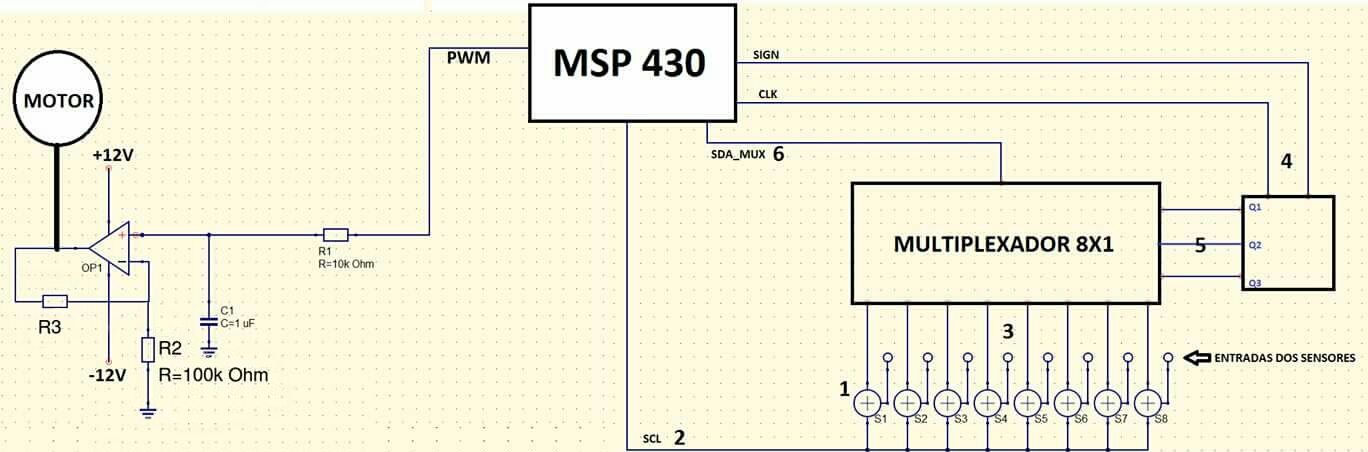
\includegraphics[scale=0.2]{figuras/mod_completo.png}
    \caption{Circuito Completo}
    \label{mod_completo}
\end{figure}

\subsection*{Detecção de Módulos Adicionais}

Um fator importante no sistema é a escalabilidade do mesmo, para que seja resiliente a má operação do usuário e a falhas, se torna necessário a detecção automática de módulos adicionais de sensores. Para a implementação desse mecanismo, sera usado o principio simples do divisor de tensão. Cada modulo possuirá uma resistência de valor igual ao de uma resistência de referencia pre-determinada $R_{ref1}$. O circuito da figura \ref{circ-exp} sera usado para essa função:

\begin{figure}[htbp]
    \centering
        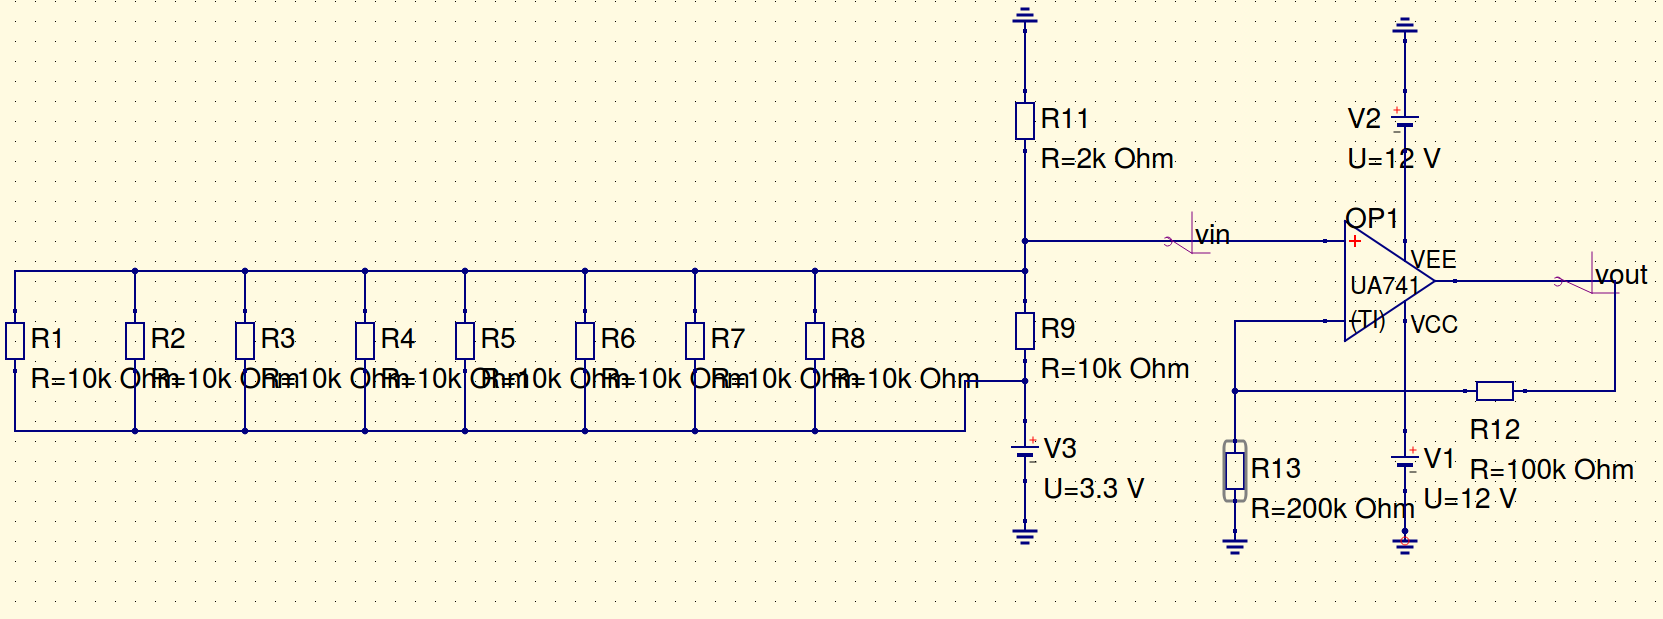
\includegraphics[scale=0.1]{figuras/exp-board-detection.png}
    \caption{Circuito de Expansao}
    \label{circ-exp}
\end{figure}

Os módulos de expansão (representados pelas resistências de $R_{1}$ a $R_{8}$ serão conectados em paralelo e assim a resistência da combinação dos mesmo sera cada vez menor, e consequentemente maior sera a tensão de entrada no amplificador operacional. Essas resistências dos módulos devem ser sempre de valor o mais próximo possível de $R_{ref1}$ para garantir o funcionamento. O amplificador esta na configuração não inversora, e possui ganho representado na equação \ref{ganho-simples}:

\begin{equation}\label{ganho-simples}
A=\frac{ R_{a} }{ R_{b} } + 1
\end{equation}

A resistência equivalente da combinação dos módulos com a resistência de referencia é dado pela equação \ref{resEq}:

\begin{equation}\label{resEq}
ResEq = \left( \frac{ N_{sensores} + 1 }{ R_{ref1} } \right)^{-1}  = \frac{ R_{ref1} }{ N_{sensores} + 1 }
\end{equation}

Consequentemente a tensão de saída sera dada por:

\begin{equation}\label{resEq}
V_{out} = \frac{R_{ref1}}{\frac{ R_{ref2} }{ N_{sensores} + 1 } + R_{ref2}} \cdot V_{ref} \left( \frac{ R_{a} }{ R_{b} } + 1\right)
\end{equation}

Manipulando a equação \ref{resEq} podemos determinar $N_{sensores}$ a partir dos outros parâmetros:

\begin{equation}\label{Nsen1}
N_{sensores} = \left[ \left( \frac{R_{ref1}}{R_{ref2}} \right) \cdot \left( \frac{V_{out}}{V_{ref} \left( \frac{ R_{a} }{ R_{b} } + 1\right) - V_{out}} \right) \right] - 1
\end{equation}

A equação \ref{Nsen1} fornece valores aproximados para a quantidade de sensores, para tornar esse valor valor mais preciso foram adicionados dois componentes na mesma: FatorAjuste (aplica um ganho em porcentagem na equação \ref{Nsen1} para compensar a imprecisão dos valores das resistências) e \textit{\% 1}(realiza a operação de quociente por 1, isto é, elimina a parte decimal para obter o valor exato do numero de módulos de expansão)

\begin{equation}\label{Nsen2}
N_{sensores} =
\left(
    \left\lbrace
        \left[
            \left( \frac{ R_{ref1} }{ R_{ref2} } \right)
            \cdot
            \left( \frac{V_{out}}{ V_{ref} \left(
                \frac{ R_{a} }{ R_{b} } + 1
            \right)
             - V_{out}} \right)
        \right] - 1
    \right\rbrace \cdot \left( 1 + FatorAjuste \right)
\right) \% 1
\end{equation}

Foram determinados os seguintes valores para os componente e parâmetros:
\begin{itemize}
    \item $R_{ref1} = 10k\Omega$
    \item $R_{ref2} = 2k\Omega$
    \item $R_{a} = 100k\Omega$
    \item $R_{b} = 200k\Omega$
    \item $V_{ref}$ = 3.3V
\end{itemize}

A equação \ref{Nsen2} pode ser reescrita substituindo pelos valores definidos da seguinte forma:

\begin{equation}\label{Nsen3}
N_{sensores} =
\left(
    \left\lbrace
            \frac{ 6 \cdot V_{out} - 4.95 }{4.95
             - V_{out}}
    \right\rbrace \cdot \left( 1 + FatorAjuste \right)
\right) \% 1
\end{equation}

O circuito da figura \ref{circ-exp} foi simulado usado o software QUCS (Quite Universal Circuit Simulator) e usando a equação \ref{Nsen3} com um fator de ajuste de 1$\%$ foram obtidos os seguintes resultados na tabela \ref{result-nsen3}.

\begin{table}[]
\centering
\caption{Resultados Experimentais}
\label{result-nsen3}
\begin{tabular}{|l|l|l|l|}
\hline
Módulos Conectados & $V_{out} (V)$ & $N_{modulos}$ & $N_{modulos}  \%  1$ \\ \hline
0 & 0.83 & -0.0004 & 0 \\ \hline
1 & 1.43 & 1.0128 & 1 \\ \hline
2 & 1.87 & 2.0070 & 2 \\ \hline
3 & 2.22 & 3.0023 & 3 \\ \hline
4 & 2.50 & 4.0400 & 4 \\ \hline
5 & 2.73 & 5.0633 & 5 \\ \hline
6 & 2.92 & 6.0794 & 6 \\ \hline
7 & 3.08 & 7.0910 & 7 \\ \hline
8 & 3.21 & 8.0461 & 8 \\ \hline
\end{tabular}
\end{table}

\subsection*{Conversor Digital para Analógico}
\subsubsection*{Introdução}
O inversor de frequência escolhido para o projeto pode ser controlado usando uma referência analógica de tensão ou de corrente para aferir a velocidade do motor a ser controlado. Foi definido que será usada a referencia analógica de tensão pois a mesma e controlada por uma tensão que varia de 0 a 10V enquanto a referencia por corrente se da dentro de um intervalo de 4 a 20mA, o circuito de condicionamento de sinais para o intervalo de tensão acima e mais simples e robusto do que o de corrente baseado no microprocessador escolhido (MSP430). O microcontrolador não possui uma saída de tensão analógica porém possui saídas capazes de serem utilizadas com PWM (Pulse Width Modulation), usando um simples circuito de conversão de sinais se torna possível converter uma saída de tensão digital de PWM que varia de 0 a 3.3V (tensão máxima e mínima de saída do MSP430) em uma saída de tensão analógica de 0 a 10V.
\subsubsection*{PWM}
Um sinal PWM é formado por uma série de pulsos de amplitude e frequência fixas porém com largura dos pulsos variável. Assim como é possível transmitir um sinal analógico por primeiramente modulando o sinal em uma onda portadora e depois removendo a portadora e ficando apenas com o sinal, também é possível transmitir uma tensão analógica modulada em uma portadora digital. Essa tensão analógica pode ser facilmente extraída do sinal modulado um usando um filtro passa-baixas.
\begin{figure}[htbp]
    \centering
    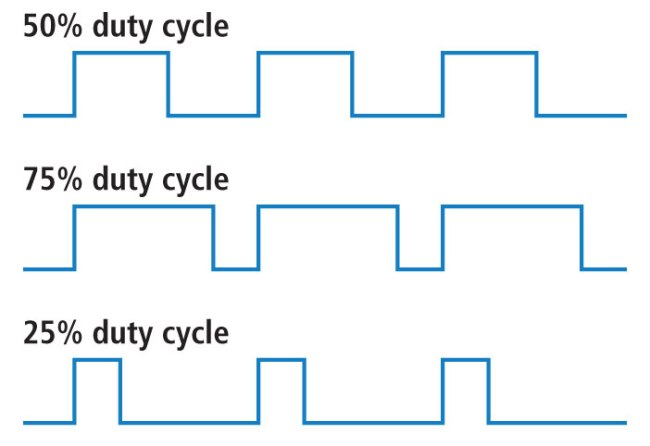
\includegraphics[scale=0.3]{figuras/duty_cycle.jpg}
    \caption{Duty Cycle}
    \label{duty_cycle}
\end{figure}
Em PWM, o tempo em que o sinal fica em nível lógico alto ou baixo não costuma ser muito usado, o mais comum é classificar o sinal de acordo com seu duty-cycle. A relação entre duty-cycle, amplitude e tensão nominal de saída do DAC se torna bem intuitiva. No domínio da frequência, um filtro passa-baixas suprime componentes de alta frequência, consequentemente no domínio do tempo isso acaba "amaciando" o sinal e de certa forma tirando uma media do sinal. Filtrar um sinal PWM com um filtro passa-baixas extrai seu valor médio de tensão. Se por exemplo o duty-cyle de um sinal for 50\% com máximo e mínimo respectivamente em 5 e 0V, após o sinal ser passado pelo filtro o sinal de saída ira possuir uma saída de 2.5V.

\begin{equation}\label{calc-duty-cycle}
    D=\frac{ PW }{ T } \cdot 100 \%
\end{equation}

Na Equação \ref{calc-duty-cycle}, D é o valor do duty cyle em percentagem, PW a largura do pulso e T o período total do sinal.

\begin{equation}\label{calc-analog-voltage}
    V_{out}=\frac{ Pw }{ T } \cdot V_{max}
\end{equation}

A Equação \ref{calc-analog-voltage} calcula a tensão de saída aproximada do sinal após o filtro passa-baixas. Na mesma $V_{out}$ é a tensão de saída, PW a largura do pulso e T o período total do sinal e $V_{max}$ é a tensão do sinal PWM quando em nível lógico alto.

\subsubsection*{Filtro passa-baixas}

Existem duas condições a serem consideradas no projeto do filtro passa-baixas: O tempo de estabilização e o ripple. Tempo de estabilização é o tempo que o sinal leva para chegar ao nível analógico desejado, já o ripple é o ruído residual da filtragem do sinal do saída. Uma frequência de corte baixa gera um sinal com pouco ripple porém aumenta o tempo de estabilização, consequentemente uma frequência de corte mais alta produz um ripple muito grande e um tempo de estabilização curto. O que deve ser feito é escolher uma frequência de corte que gera um ripple menor que a resolução da entrada analógica do inversor de frequência (vale lembrar que resolução é a menor variação de tensão que o dispositivo pode ler). \\

As especificações para projeto do filtro conversor são:

\begin{itemize}
    \item Frequência PWM de entrada = 100KHz
    \item Resolução da entrada do inversor (ripple máximo) = 9.76mV
    \item Tempo de estabilização = 0.1s
    \item Ganho de Tensão = 3
\end{itemize}

O circuito a ser usado será o da Figura \ref{active-lpf}:

\begin{figure}[htbp]
    \centering
    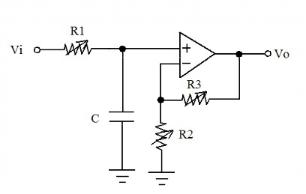
\includegraphics[scale=0.3]{figuras/lpf.jpg}
    \caption{Filtro passa-baixas ativo}
    \label{active-lpf}
\end{figure}

A frequência de corte para o filtro é dada pela Equação \ref{cuttof-frequency}

\begin{equation}\label{cutoff-frequency}
    f_{c}=\frac{ 1 }{ 2 \Pi \cdot R_{1}\cdot C } \cdot V_{max}
\end{equation}

Os resistores $R_{2}$ e $R_{3}$ controlam o ganho do filtro que é dado pela Equação \ref{ganho_alpf}

\begin{equation}\label{calc-analog-voltage}
    G= 1 + \frac{ R_{3} }{ R_{2} }
\end{equation}

Foram usados os seguintes componentes para o circuito:

\begin{itemize}
    \item $R_{1}=10k\Omega$
    \item $R_{2}=100k\Omega$
    \item $R_{3}=200k\Omega$
    \item C=1uF
\end{itemize}

Esse circuito gera uma frequência de corte de aproximadamente 16Hz, um ripple de 2.4mV, um tempo de estabilização de 0.02s e um ganho de tensão igual a 3. Dessa forma atende todas os requisitos de funcionamento. A Figura \ref{filter_out} mostra a saída sem ripple.

\begin{figure}[htbp]
    \centering
    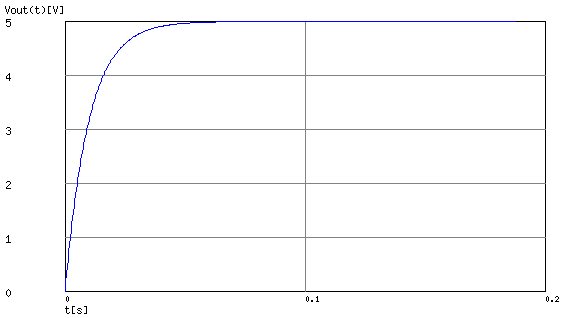
\includegraphics[scale=0.3]{figuras/ripple-lpf.png}
    \caption{Gráfico TensãoxTempo filtro passa baixas}
    \label{filter_out}
\end{figure}





\section{Projeto de Processamento e Interface}

\label{desenvolvimento_processamento}

Nesta seção é descrito o detalhamento da solução do módulo de interface/processamento, resultante das duas primeiras fases, 
e o seu projeto e construção, resultante da Fase 03. Além disso, a visão da solução e da arquitetura estão
documentadas nos Apêndices \ref{documento_visao} e \ref{documento_arquitetura}.

\subsection{Detalhamento da Solução} \label{software:detalhamento_solucao}

O detalhamento da solução para a frente de interface/processamento pode ser sumarizado nos itens abaixo. A solução completa definida nas 
  Fases 01 e 02 pode ser vista no \href{https://drive.google.com/file/d/0B5InkGKx6O-MR1B3eVYzZFpjQ3c/view?usp=sharing}{Relatório 1}.
% Esta subseção apresenta a visão da solução da parte de processamento e interface referentes a Software, e
% integração com a frente de Eletro-eletrônica. A intenção desta frente é apresentar a visão da arquitetura do sistema,
% bem como será o fluxo de dados entre usuário até chegar ao sistema. A intenção é transmitir as decisões significativas do 
% ponto de vista da arquitetura de baixo e alto nível que foram tomadas de acordo com as necessidades do sistema.

% \subsubsection*{\textbf{Escopo}}

% A arquitetura que foi idealizada fundamenta a base para a construção do produto, expressando como o sistema deverá se 
% comportar em suas interações, bem como o nível de abrangência da aplicação em quesitos de limitação e qualidade.

% O escopo deste projeto vai de encontro em cobrir os aspectos de comunicação entre usuário e sistema, bem como o tratamento
% dos dados embarcados. Para isso, este será apresentado o dimensionamento do sistema, tanto em alto nível, com relação à aplicação 
% web, quanto em baixo nível, referente a rotina de comunicação entre Raspberry PI e Arduino e a rotina de processamento de dados.

% \subsubsection*{\textbf{Representação da Arquitetura}}

% A arquitetura da aplicação utiliza de padrões que organizam e aperfeiçoam o desenvolvimento dentro do paradigma de Orientação a 
% Objetos e adicionalmente, a persistência e o consumo de dados.

% Quanto à camada de alto nível, para o corrente projeto da bancada de vibrações, optou-se por desenvolver uma aplicação web para que 
% o usuário possa fornecer inputs de controle para operação da bancada e também, visualizar os resultados do ensaio realizado.

% É válido ressaltar que para fins de boa performance da aplicação web, foram consideradas abordagens para o projeto de aplicativos 
% da Web fracamente acoplados. Nesse cenário, o estilo REST (Representational State Transfer - Transferência de Estado Representacional)
% foi adotado.

% Roy Fielding, um dos idealizadores do estilo REST,  afirma que o estilo REST enfatiza a escalabilidade das interações entre 
% componentes e componentes intermediários para reduzir a latência da interação.

% De uma forma geral, vale notar que tudo na Web (páginas, imagens, entre outros) são a essência de um recurso \footnote{http://www.ibm.com/developerworks/br/library/j-rest/}.
% O fato de o REST  possuir a  característica de contar com recursos nomeados em vez de mensagens facilita o fraco acoplamento 
% no design da aplicação.

% Logo abaixo, é possível contemplar uma figura esquemática da arquitetura geral do sistema.

% \begin{figure}[!ht]
% \centering
% 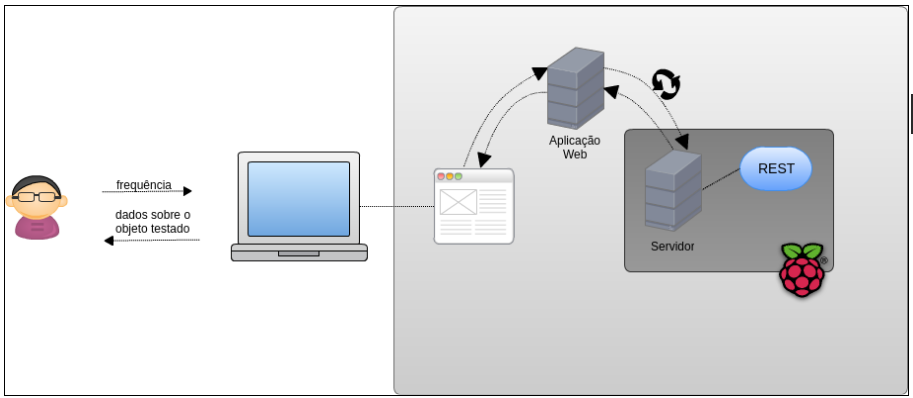
\includegraphics[scale=0.5]{figuras/arquitetura_sistema.png}
% \caption{Esquema geral da arquitetura do sistema. Fonte: Autores}
% \label{fig:arquitetura_sistema}
% \end{figure}

% Para a realização dos testes na bancada, o usuário poderá determinar a frequência de vibração e o tempo de funcionamento da 
% bancada por meio da interação com uma aplicação web. Durante e após a execução dos testes, o usuário poderá visualizar os dados
% coletados pelos sensores.

% A aplicação web fará requisições, através de uma rotina, para um servidor que provê serviços REST. Este servidor será disponibilizado
% por uma Raspberry Pi. É valido ressaltar que a comunicação entre aplicação web e o Raspberry PI funcione é necessário que o mesmo 
% esteja com acesso a internet para que ele possa receber e enviar as requisições para a aplicação web.

% Adicionalmente, os serviços REST consultarão os dados coletados e persistidos em uma base de dados SQLite , que também será hospedado
% na Raspberry Pi.

% Para a camada de baixo nível será desenvolvido uma rotina responsável por enviar, receber dados entre Arduino e Raspberry PI, bem 
% como disponibilizar os dados recebidos na forma de arquivos que serão utilizados pela aplicação para que o usuário consiga ver os 
% resultados das ações que foram aplicadas no sistema. Toda essa transmissão de dados será feita com a interface UART \footnote{http://www.raspberry-projects.com/pi/programming-in-c/uart-serial-port/using-the-uart}
% (Universal Asynchronous Receiver Transmitter - Transmissor Receptor Assíncrono Universal), via serialização de dados.

% Os dados de resultados que chegarem do Arduino para a Raspberry PI, serão tratados pela rotina de comunicação de forma a 
% disponibilizar esses dados brutos em arquivos. Estes arquivos serão lidos por uma rotina que terá como objetivo realizar o 
% processamento dos dados e logo em seguida a realização do parser (leitura dos dados nos arquivos e a gravação deles no banco 
% de dados embarcado) desses dados no banco de dados local.

% \begin{figure}[!ht]
% \centering
% 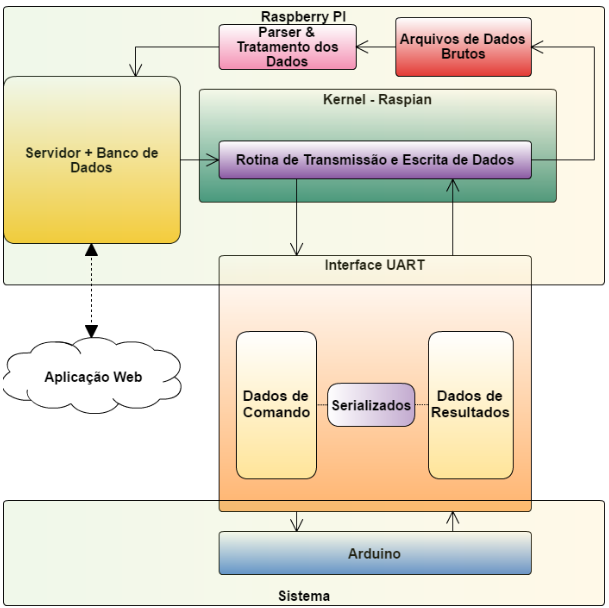
\includegraphics[scale=0.5]{figuras/sistema.png}
% \caption{Camada baixo nível do sistema, responsável pela comunicação entre a aplicação web e o sistema da bancada de vibração}
% \label{fig:sistema}
% \end{figure}

% Por fim, vale destacar que a rotina é o meio de integração entre Software e Eletrônica o qual teremos uma comunicação
% de baixo nível pela porta serial e os resultados obtidos entregues na forma de arquivos, ou seja, separando a comunicação 
% entre Hardware e a aplicação. Serão utilizados rotinas para tratamento dos dados de acordo com a necessidade do usuário em 
% visualizar os dados de resultados derivados.

% \subsubsection*{\textbf{Restrições Arquiteturais}}
% Com o objetivo de se criar um sistema confiável, estabeleceu-se que deverá ser feita uma avaliação dos componentes mais críticos 
% e deverão ser elaborados testes unitários para assegurar o bom funcionamento destes módulos.

% Adicionalmente, dentre as opções de linguagens de programação disponíveis para desenvolvimento de aplicações web, e do parser e 
% tratamento dos dados brutos, optou-se pela linguagem Python e para a camada de baixo nível será utilizado a linguagem C para o 
% desenvolvimento  das rotinas de comunicação entre Raspberry PI e Arduino. O desenvolvimento da aplicação web e dos serviços REST 
% será feito com o auxílio de recursos providos pelo framework Django \footnotemark, que oferece uma alta produtividade no 
% desenvolvimento.
% \footnotetext{https://www.djangoproject.com/}

% A linguagem de programação Python possui uma excelente performance, especialmente considerando que o hardware a ser utilizado 
% para disponibilizar o servidor REST possui recursos de processamento bem limitados. Além disso, a linguagem de programação Python 
% possui uma alta produtividade associada.

% Outro aspecto vantajoso da linguagem é vasta disponibilidade de bibliotecas para tratamento de informações, especialmente cálculos
% matemáticos, que serão amplamente utilizados no sistema para uso integrado com a bancada de vibrações.
% \newpage
% \subsubsection*{\textbf{Requisitos Levantados}}
% A partir do escopo definido no projeto foram elicitados alguns requisitos de forma macro, estes podem ser vistos na 
% Figura \ref{backlog_produto} que representa os \textit{Backlogs} do Produto para as duas aplicações.

% \begin{figure}[H]
% \centering
% \label{backlog_produto}
% 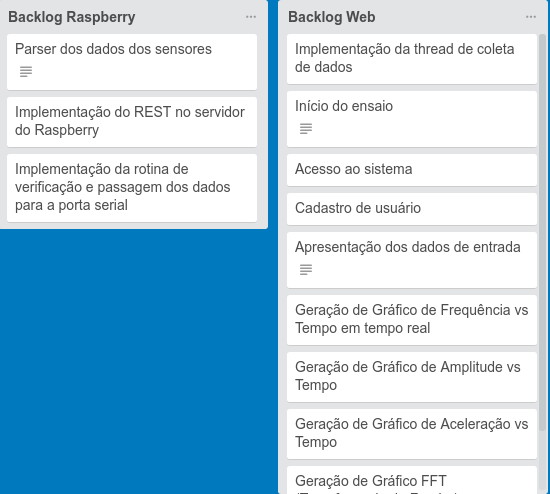
\includegraphics[keepaspectratio=true,scale=0.55]	{figuras/backlog_produto.png}
% \caption{\textit{Backlogs} das aplicações do projeto}
% \end{figure}

% \subsubsection*{\textbf{Protótipo da Solução Web}}

% Com o intuito de visualizar a solução Web foi desenhado um protótipo de alta fidelidade da aplicação Web. 
% As telas podem ser vistas no \href{https://drive.google.com/file/d/0B5InkGKx6O-MR1B3eVYzZFpjQ3c/view?usp=sharing}{Relatório 1}. 

\subsection{Projeto e Construção}

Nesta subseção é apresentado o projeto e construção do sistema proposto na Subseção \ref{software:detalhamento_solucao}, bem
como as mudanças realizadas no que foi proposto.

\subsubsection*{\textbf{Mudanças - Rotinas de Comunicação}}

A camada de software na aplicação Web foi desenvolvida em \textit{Python}, bem como a camada de servidor de comunicação com a aplicação na 
\textit{Raspberry}. Como foi relatado, os membros do grupo naquele momento haviam chegado ao consenso de utilizar a linguagem C para integrar 
com \textit{Python}, que seria utilizado nas rotinas de comunicação entre \textit{Raspberry} e os microcontroladores da baixa aplicação.

Durante o desenvolvimento das rotinas de comunicação, foi-se percebendo que não havia necessidade de que o mesmo fosse desenvolvida 
usando tal linguagem, considerando que a linguagem C é uma linguagem de baixo nível normalmente utilizada para ter um maior controle sobre o 
hardware, que não é o caso. Levando em consideração este fato, foi levantada a hipótese de utilização do módulo de comunicação serial que o próprio 
\textit{Python} oferece, e para isso foi realizado uma lista de prós e contras a cerca da linguagem no desenvolvimento das rotinas de comunicação.

Utilizando a linguagem C para o desenvolvimento das rotinas de comunicação possui as seguintes vantagens:

\begin{itemize}
    \item A linguagem C é uma linguagem de baixo nível, ou seja, oferece um maior controle do hardware, e te da possibilidade de manipulações com \textit{bytes} em uma maior flexibilidade do que as outras linguagens com exceção da linguagem \textit{ASSEMBLY}.
    \item Com a linguagem C é possível desenvolver o sistema de forma a se proteger contra falhas críticas, impedindo de repassar erros de baixo nível para a camada de alto nível.
    \item A linguagem C realiza processamentos mais velozes em comparação com as outras linguagens como \textit{Python}, dentre outras, se tornando uma excelente ferramenta para manipulação de \textit{bytes}.
\end{itemize}

Desvantagens da utilização da linguagem C para o desenvolvimento das rotinas de comunicação:

\begin{itemize}
    \item Por ser uma linguagem de baixo nível com uma alta tipagem, o trabalho de desenvolver uma rotina de comunicação serial usando recursos da camada de hardware se tornam bastante complexos.
    \item Na arquitetura proposta no primeiro ponto de controle, as rotinas de escrita e leitura de dados funcionariam da seguinte maneira, a escrita iria ler um arquivo, em seguida iria apagá-lo enviaria este dado para o sistema de controle, e no sistema de leitura, seria aberta a porta seria para leitura dos \textit{bytes}, que seriam decodificados e transcritos num arquivo para serem lidos por uma rotina \textit{Python} para escrever no banco de dados. Ou seja, a integração possui uma alta complexidade.
    \item Apesar da linguagem C ser mais rápida que \textit{Python}, não existe necessidade das rotinas serem desenvolvidas em tal linguagem, pois a diferença de velocidade de escrita e leitura para comunicação serial é bem mínima levando em consideração ao que \textit{Python} também faz.
\end{itemize}

Vantagens em utilizar \textit{Python} para o desenvolvimento das rotinas de comunicação:

\begin{itemize}
    \item Python possui uma baixa tipagem.
    \item Possui uma biblioteca de comunicação serial que realiza a abstração do jeito que o desenvolvedor quiser (seja controlar em baixo nível, ou em alto nível com uma abstração do controle).
    \item Fácil integração com \textit{RESTful} do \textit{Django} que é realizado em \textit{Python}.
    \item Elimina necessidade de escrever e ler em arquivos, pois os métodos podem ser carregados pelo \textit{REST} diretamente, assim o \textit{REST} terá o controle total da comunicação.
    \item Não existe necessidade de manipular leitura e escrita de bytes, devida a abstração da biblioteca.
    \item \textit{Python} é uma linguagem melhor para manipulação de dados, e permitirá a escrita dos dados recebidos diretamente no banco de dados do servidor da \textit{Raspberry}, que a aplicação irá ler.
\end{itemize}

Desvantagens da linguagem \textit{Python} para o desenvolvimento das rotinas de comunicação:

\begin{itemize}
    \item \textit{Python} é uma linguagem interpretada e mais lenta em comparação a linguagem C.
    \item Não fornece um controle maior em comparação as linguagens de baixo nível.
\end{itemize}

Com a nova mudança então, a única linguagem de programação que está sendo utilizada neste projeto é a linguagem \textit{Python}, e em virtude 
desta mudança, a arquitetura mudou um pouco agora sendo nesse novo estilo.

\begin{figure}[H]
\centering
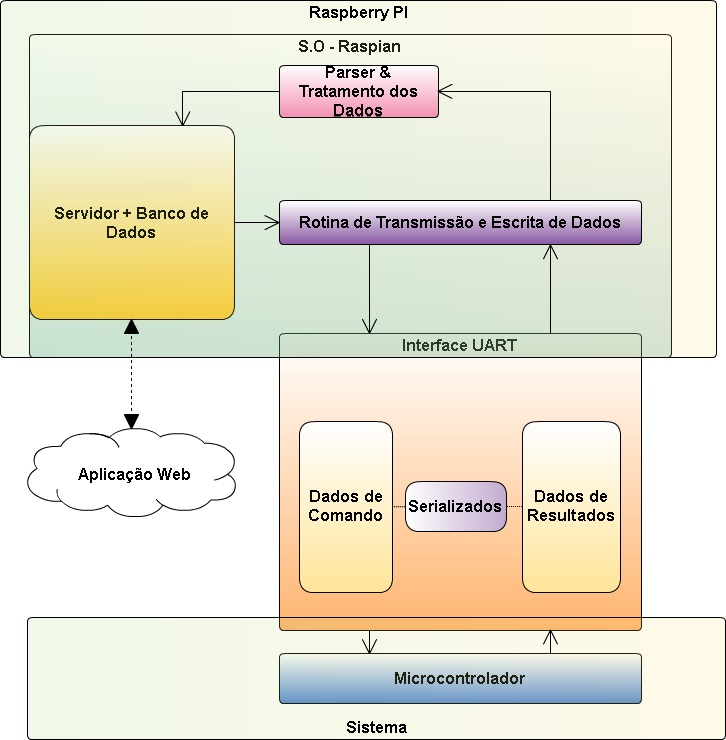
\includegraphics[keepaspectratio=true,scale=0.7]{figuras/nova_arquitetura.png}
\label{fig:nova_arquitetura}
\caption{Nova arquitetura com a mudança da linguagem implementada - Fonte: Autor}
\end{figure}

\subsubsection*{\textbf{Protocolo de Comunicação}}

As rotinas de comunicação são as pontes pela qual a frente de software irá se comunicar com a frente de eletroeletrônica e com o resto do sistema. 
Para que a comunicação seja estabelecida, foi necessário estabelecer um padrão de comunicação de acordo com ambas as frentes, de forma que a comunicação 
ocorra com sucesso e sem surpresas. Foi definido então um protocolo de comunicação ao qual deverá ser respeitado entre a frente de software e eletrônica, 
durante a transmissão de dados via serial.

Com a mudança da arquitetura, acabou facilitando a integração das rotinas de comunicação e escrita com parser e com o servidor e nos permitiu formalizar 
um protocolo bem simples para comunicação entre sistema de controle e sistema da aplicação.

Protocolo de comunicação é descrito da seguinte forma: Ele é dividido em duas partes, em protocolo de controle e protocolo resposta.

\begin{itemize}
    \item Protocolo de Controle
    \begin{itemize}
        \item É definido por \textit{flags} que permitirão que o sistema realize ações pré-definidas.
    \end{itemize}
    \item Protocolo de Resposta
    \begin{itemize}
        \item É definido a \textit{STRING} de resposta que o sistema de controle enviará para a camada de alto nível no caso a \textit{Raspberry} via 
        comunicação serial.
    \end{itemize}
\end{itemize}

\begin{figure}[H]
\centering
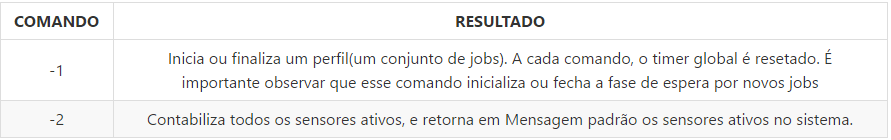
\includegraphics[keepaspectratio=true,scale=0.7]{figuras/protocolo_controle.png}
\label{fig:protocolo_controle}
\caption{Protocolo de Controle com \textit{flags} já definidas - Fonte: Autor}
\end{figure}

\begin{figure}[H]
\centering
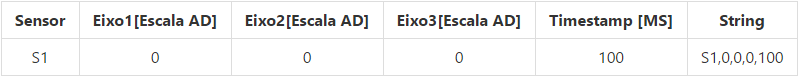
\includegraphics[keepaspectratio=true,scale=0.8]{figuras/protocolo_string.png}
\label{fig:protocolo_string}
\caption{Protocolo de Resposta e o formato da String que chegará ao sistema - Fonte: Autor}
\end{figure}

Com esse padrão definido, o usuário definirá um determinado número de \textit{jobs} (cada \textit{job} representa uma frequência com uma duração de tempo, 
e um conjunto de \textit{jobs} define um ensaio) que serão executados ao longo do ensaio. Ao executar o ensaio, o resultado dos sensores irão ser 
repassados na escala entre 0 a 1024 em AD (\textit{Analogic Digital}), sendo 0AD igual a 0G e 1024AD igual a 16G, ou seja, com uma regra de três simples,
determinará as acelerações dos pontos de acordo com a frequência estabelecida e, por fim, esses dados passarão pelo processamento, para serem salvos no 
banco de dados da \textit{Raspberry}.

Um dos objetivos ao obter a \textit{timestamp} a qual foi obtido o resultado pelo sensor, será para realizar o mapeamento dos \textit{jobs} de acordo 
com o ensaio, para ordenar e saber quais dados pertencem a quais \textit{jobs}.

Na Figura \ref{fig:diagrama_sequencia_pc2}, mostra um diagrama de sequência entre usuário, a aplicação web, o servidor da \textit{raspberry}, sobre 
como é tratado o \textit{input} e o \textit{output} do sistema como um todo entre as frentes da software e eletrônica.

\begin{figure}[H]
\label{fig:diagrama_sequencia_pc2}
\centering
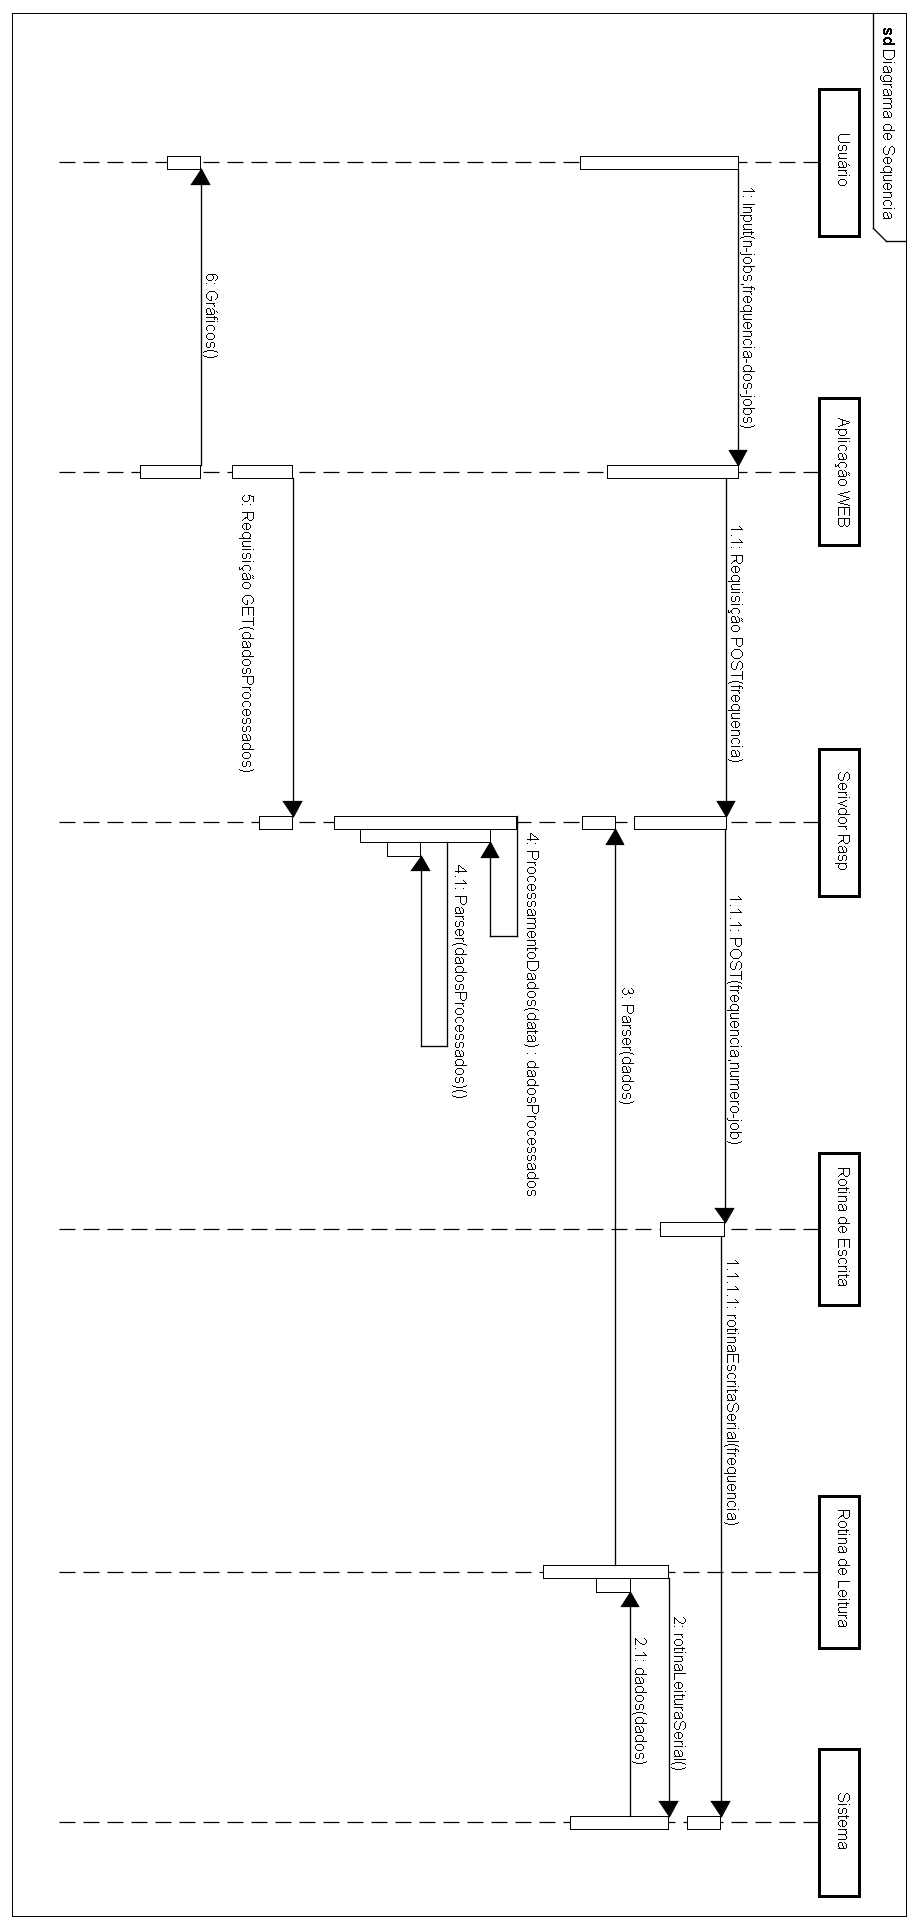
\includegraphics[keepaspectratio=true,scale=0.5]{figuras/diagrama_sequencia_pc2.png}
\caption{Diagrama de sequência - Fonte: Autor}
\end{figure}

\subsubsection*{\textbf{Arquitetura das Rotinas de Comunicação e Parser}}

Para realização das rotinas de comunicação e parser, a equipe de software contou com um simulador. O simulador, construído pela frente de eletroeletrônica, 
consiste em um \textit{Arduino} que simula o comportamento da entrada e saída de dados que o sistema da \textit{Raspberry} terá de comunicar. Com isso 
então, foi possível realizar o desenvolvimento das rotinas de comunicação em \textit{Python}, bem como iniciar também o \textit{Parser}.

O \textit{Parser} foi construído utilizando a base de dados que o próprio \textit{Django} oferece, que no caso é o \textit{SQLITE3}, foi simulado uma 
entrada de uma \textit{String} seguindo o protocolo de comunicação e em seguida essa \textit{String} é tratada para que seja guardada no banco de dados 
da aplicação local. O primeiro passo consiste em conectar no banco de dados, e em seguida realizar o tratamento dos dados em uma lista de forma a 
averiguar se os dados estão corretos de acordo com a entrada de elementos das tabelas no banco de dados. O próximo passo então insere os dados da lista 
no banco de dados, usando o método \textit{inserting acceleration} e assim por diante para os outros dados.

É importante ressaltar que o processamento está planejado para o ponto de controle 3, que utilizará essa base de dados local para realizar os cálculos 
e então inserir os dados de acordo com as tabelas de velocidade, amplitude e frequência, que serão utilizados pela aplicação web.

Com relação as rotinas de entrada e saída de dados, foi utilizado o \textit{Arduino} para fins de teste de comunicação. A frente de eletroeletrônica 
desenvolveu uma rotina que é executada no \textit{Arduino} que conseguia simular a entrada e saída de dados com o comportamento similar ao esperado. 
Então utilizado a biblioteca serial que é padrão em \textit{Python}, foi possível construir métodos abstraindo o controle da comunicação serial em baixo
nível para um alto nível, e conectá-los as rotinas que guardarão os dados, no caso o \textit{Parser}.

Para comunicação com a malha fechada de controle do sistema, foi desenvolvido o \textit{Pyserial}. Uma classe que abstrai os principais métodos da 
biblioteca padrão do \textit{Python} chamada serial. Com essa biblioteca foi possível inicializar os valores como \textit{BAUDRATE} (Taxa de transmissão),
\textit{Timeout} e a porta serial de entrada e saída dos dados. A classe também conta com um método simples que acumula os resultados de leitura da porta 
serial em uma grande lista que será utilizada pelo \textit{Parser} para o tratamento dos dados resultantes para que eles possam ser guardados no banco de 
dados. A classe também conta com um tratamento de exceções para evitar que as exceções subam em nível de usuário.

O \textit{RoutinesUtil}, é uma classe que faz parte da solução em \textit{Django} no pacote de classes e ele é responsável por definir o comportamento 
da rotina. Nesta classe são definidas as rotinas de leitura de dados resultantes, dos sensores ativos e da escrita de controle do sistema. Ela utiliza 
as classes \textit{Pyserial} e \textit{Parser} para abrir a porta serial, ler os dados, fechar a porta serial e gravar no banco de dados da aplicação do 
servidor, que mandará para aplicação Web.

A integração entre eletroeletrônica e software vem com as rotinas que irão se comunicar com a malha fechada de controle do sistema e com a 
\textit{Raspberry} da aplicação, responsáveis por armazenar os resultados e processá-las para a aplicação web. Na imagem abaixo você poderá verificar 
o diagrama de classes parcial das rotinas de comunicação em integração com o \textit{Django} da \textit{Raspberry} e seus respectivos métodos.

\begin{figure}[H]
\centering
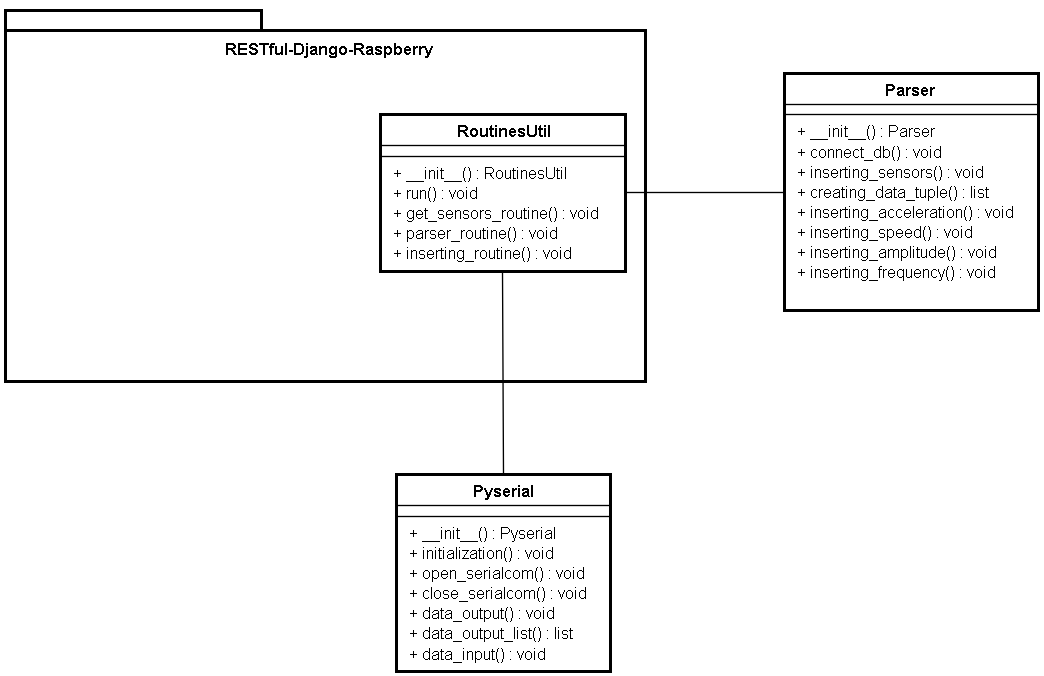
\includegraphics[keepaspectratio=true,scale=0.65]{figuras/uml_routines_parser.png}
\label{fig:uml_routines_parser}
\caption{Diagrama de Classes Parcial das Rotinas de Comunicação e Parser, integrados ao \textit{Django} - Fonte: Autor}
\end{figure}

\subsubsection*{\textbf{Processamento dos Dados}}

A integral é uma das mais importantes ferramentas matemáticas e que aparece com frequência na solução de problemas e no cálculo de grandezas 
na engenharia e na ciência \cite{metodos_numericos}.

Na engenharia, há situações que envolvem dados experimentais ou de teste, nos quais uma grandeza física a ser determinada pode ser expressa 
como a integral de outras grandezas medidas. Assim, é válido ressaltar que o integrando pode ser uma função analítica ou um conjunto de pontos
discretos (dados tabulados).

Quando se tem um integrando expresso de forma que a integral pode ser facilmente calculada, pode-se obter analiticamente o valor da integral 
definida. A integração numérica faz-se necessária quando a integração analítica é difícil, ou mesmo impossível, e quando o integrando é fornecido
como um conjunto discreto de pontos \cite{metodos_numericos}.

Este é o caso da Bancada de Vibrações Mecânicas que está sendo construída neste projeto. Os dados que se tem são o retorno da leitura dos sensores 
e assim, o integrando é fornecido como um conjunto de pontos.

A análise numérica de uma integral caracteriza-se por estimar  o número correspondente à integral de uma função entre os limites [a, b]. 
Caso seja utilizado apenas os pontos finais do intervalo, pode ser que o resultado fornecido não seja suficientemente preciso, especialmente se
o intervalo for significativamente grande ou se o integrando variar significativamente ao longo do intervalo. Dessa maneira, uma maior precisão 
pode ser obtida com o uso de um método composto, no qual o intervalo [a, b] é dividido em subintervalos menores. Assim, calcula-se a integral ao
longo de cada subintervalo e os resultados são somados para fornecer a integral completa.

É importante ressaltar que existem vários métodos disponíveis para o cálculo numérico de integrais. Esses métodos podem ser divididos em abertos 
e fechados. Os métodos de integração fechados consideram os pontos finais do intervalo e o integrando propriamente dito na fórmula que estima o
valor da integral. Já nos métodos de integração abertos, o intervalo de integração se estende além do limite especificado pelos pontos finais 
\cite{metodos_numericos}.

Devido à variedade de métodos, os principais foram analisados e verificou-se sua aplicação no âmbito do projeto. Os métodos considerados foram: 
Trapezoidal Composto, Métodos de Simpson e Quadratura de Gauss.

No {\textbf{Método Trapezoidal Composto}} a integral, ao longo do intervalo [a, b], pode ser avaliada de forma mais precisa com a subdivisão do 
intervalo, a avaliação da integral em cada um dos subintervalos e a soma dos resultados. A imagem a seguir ilustra a expansão genérica para a 
integração numérica por trapézios.

\begin{figure}[H]
\centering
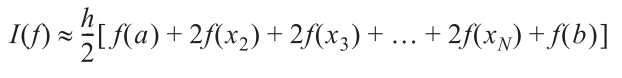
\includegraphics[keepaspectratio=true,scale=0.52]	{figuras/metodo_trapezoidal.png}
\label{fig:metodo_trapezoidal}
\caption{Integração numérica por Trapézios Acumulados - Fonte: \citeonline{metodos_numericos}}
\end{figure}

É importante notar que a fórmula do método trapezoidal composto se aplica precisamente para os casos onde os subintervalos têm uma largura h
idêntica. Outro aspecto interessante no uso desse método é que a precisão da resposta pode melhorar a partir da utilização de mais subintervalos.

O método trapezoidal aproxima o integrando por uma linha reta. De fato, seria melhor a aproximação por meio da representação do integrando 
como uma função não-linear e de fácil integração.

Há um grupo de métodos dotados desta característica, denominados \textbf{Métodos de Simpson}, utilizando polinômios quadráticos (método de
Simpson 1/3) e polinômios cúbicos, no caso do método de Simpson 3/8.

Os métodos de Simpson possuem restrições mais severas para uso. No caso do método de Simpson 1/3 composto, os subintervalos devem ser 
igualmente espaçados e o número de subintervalos no intervalo [a, b] deve ser um número necessariamente par. Com relação ao método de Simpson 
3/8 composto, além do espaçamento igual na identificação dos subintervalos, tem-se que o número de subintervalos no intervalo [a, b] deve ser 
divisível por 3.

Por fim, na \textbf{Quadratura de Gauss}, a integral também é avaliada utilizando a soma ponderada dos valores da função em pontos distintos 
ao longo do intervalo [a, b]. Nessa abordagem, são utilizados os pontos de Gauss, que, por sua vez, não são igualmente espaçados e não incluem 
os pontos finais.

Para o projeto da Bancada de Vibrações, optou-se pelo uso do método dos trapézios acumulados (método trapezoidal composto). A frente de 
controle projetou uma leitura dos dados dos sensores que garantirá intervalos de tempo igualmente espaçados, já favorecendo a aplicação de 
tal método. Outro aspecto interessante é que não será necessário controlar se o número de subintervalos é par ou se é divisível por três. 
O método dos trapézios se aplica independentemente deste aspecto.

Outro aspecto que deve ser notado é que como a massa de dados coletada a partir da leitura das medições feitas pelos sensores é grande, a
precisão do método será ainda maior.

\section{Integração dos subsistemas}

Considerando os produtos gerados nas frentes de trabalho citados nas Seções anteriores o sistema completo será integrado de acordo com
a representação da Figura \ref{fig:arquitetura_solucao}.

\begin{figure}[H]
\centering
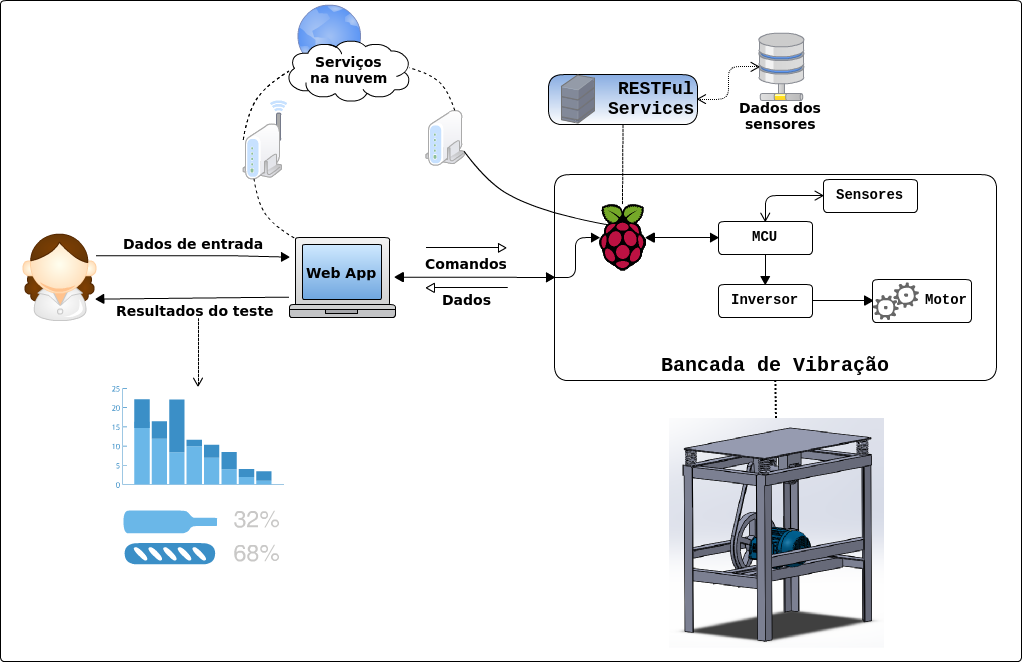
\includegraphics[scale=0.45]{figuras/arquitetura_solucao.png}
\caption{Arquitetura Geral da Solução.  Fonte: Autores}
\label{fig:arquitetura_solucao}
\end{figure}

Para iniciar um ensaio o usuário insere as frequências e tempos desejados na aplicação web, que passa essa informação
para a Raspberry através do protocolo HTTP. Na Raspberry é realizada a comunicação serial com o microcontrolador possibilitando 
a comunicação com o sistema de controle eletroeletrônico. Esse servidor estabelece comunicação com o sistema de controle
através de protocolos definidos na subseção \ref{software:protocolo}.

Com o envio das frequências estabelecidas pelo usuário para o sistema de controle, este é responsável por enviar a 
frequência ao inversor. Desse modo, ocorre a integração dos subsistemas eletroeletrônico e eletromecânico. 
O procedimento de integração contempla a interligação do sistema de controle eletroeletrônico
com o inversor que rege a velocidade do motor a partir dos bornes analógicos na forma de variações de tensão.

A integração dos subsistemas eletromecânico e de estrutura será realizada através da fixação 
do motor aos furos dedicados na estrutura e o acoplamento por meio de 
transmissão por correia entre o eixo do volante desbalanceado, fixado no mancal da superfície vibratória, com o motor 
do sistema, para que a bancada seja capaz de vibrar.

Com a integração do fluxo de controle realizada, para a coleta de dados do ensaio há a comunicação do sistema de controle eletroeletrônico com
o sistema de interface e processamento através dos protocolos definidos na subseção \ref{software:protocolo}. Os dados são coletados através
dos acelerômetros acoplados ao tampo e no objeto testado. Esses dados são enviados ao servidor da Raspberry.

Os testes a serem realizados para testar a integração dos subsistemas podem ser vistos no Apêndice \ref{documento_teste}.

\subsection*{\textbf{Protocolos - Interface/Processamento e Controle}} \label{software:protocolo}

As rotinas de comunicação são as pontes pelas quais os componentes de software do servidor que estará rodando na \textit{Raspberry} irão se
comunicar com os componentes eletroeletrônicos do sistema de controle e, consequentemente, com o resto do sistema. 
Para que a comunicação seja estabelecida é necessário estabelecer um padrão de comunicação de acordo com ambas as frentes, de forma que a comunicação 
ocorra com sucesso e sem surpresas. Foi definido então um protocolo de comunicação que deve ser respeitado pela frente de software e
eletrônica durante a transmissão de dados via serial.

Com a mudança da arquitetura ficou mais simples a integração das rotinas de comunicação e de escrita (com o parser dos dados)
com o
servidor, o que nos permitiu formalizar um protocolo bem simples para a comunicação entre o sistema de controle e o 
sistema da aplicação.

O protocolo de comunicação é dividido em duas partes: o protocolo de controle e o protocolo de resposta, que são apresentados 
abaixo.

\begin{itemize}
    \item \textbf{Protocolo de Controle}
    \begin{itemize}
        \item É definido por \textit{flags} que permitirão que o sistema realize ações pré-definidas.
    \end{itemize}
    \item \textbf{Protocolo de Resposta}
    \begin{itemize}
        \item É definida a \textit{STRING} de resposta que o sistema de controle enviará para a camada de alto nível, no caso a \textit{Raspberry}, via 
        comunicação serial.
    \end{itemize}
\end{itemize}

\begin{figure}[H]
\centering
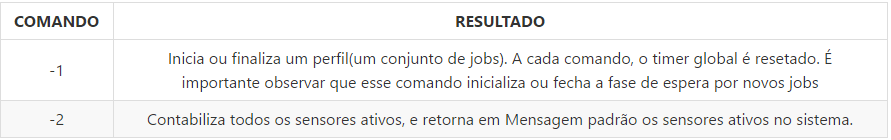
\includegraphics[keepaspectratio=true,scale=0.7]{figuras/protocolo_controle.png}
\label{fig:protocolo_controle}
\caption{Protocolo de Controle com \textit{flags} já definidas - Fonte: Autor}
\end{figure}

\begin{figure}[H]
\centering
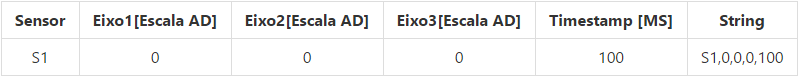
\includegraphics[keepaspectratio=true,scale=0.8]{figuras/protocolo_string.png}
\label{fig:protocolo_string}
\caption{Protocolo de Resposta e o formato da String que chegará ao sistema - Fonte: Autor}
\end{figure}

Com esse padrão definido, o usuário definirá um determinado número de \textit{jobs} (cada \textit{job} representa uma frequência com uma duração de tempo, 
e um conjunto de \textit{jobs} define um ensaio) que serão executados ao longo do ensaio. Ao executar o ensaio, os resultados dos sensores irão ser 
repassados na escala entre 0 a 1024 em AD (\textit{Analogic Digital}), sendo 0AD igual a 0G e 1024AD igual a 16G. Para determinar a aceleração a 
partir dessa escala basta utilizar uma regra de três simples. Por fim, esses dados passarão pelo processamento para serem persistidos no
banco de dados da \textit{Raspberry}.

Um dos objetivos ao obter a \textit{timestamp} a qual foi obtido o resultado pelo sensor é a necessidade de identificar e mapear os
\textit{jobs} de acordo com o ensaio, para ordenar e saber quais dados pertencem a quais \textit{jobs}.

A Figura \ref{fig:diagrama_sequencia_pc2} mostra um diagrama de sequência que apresenta a interação entre usuário, a aplicação web e o servidor da \textit{raspberry},
ilustrando como é tratado o \textit{input} e o \textit{output} do sistema como um todo entre os componentes de software e de eletrônica.

\begin{figure}[ht]
\label{fig:diagrama_sequencia_pc2}
\centering
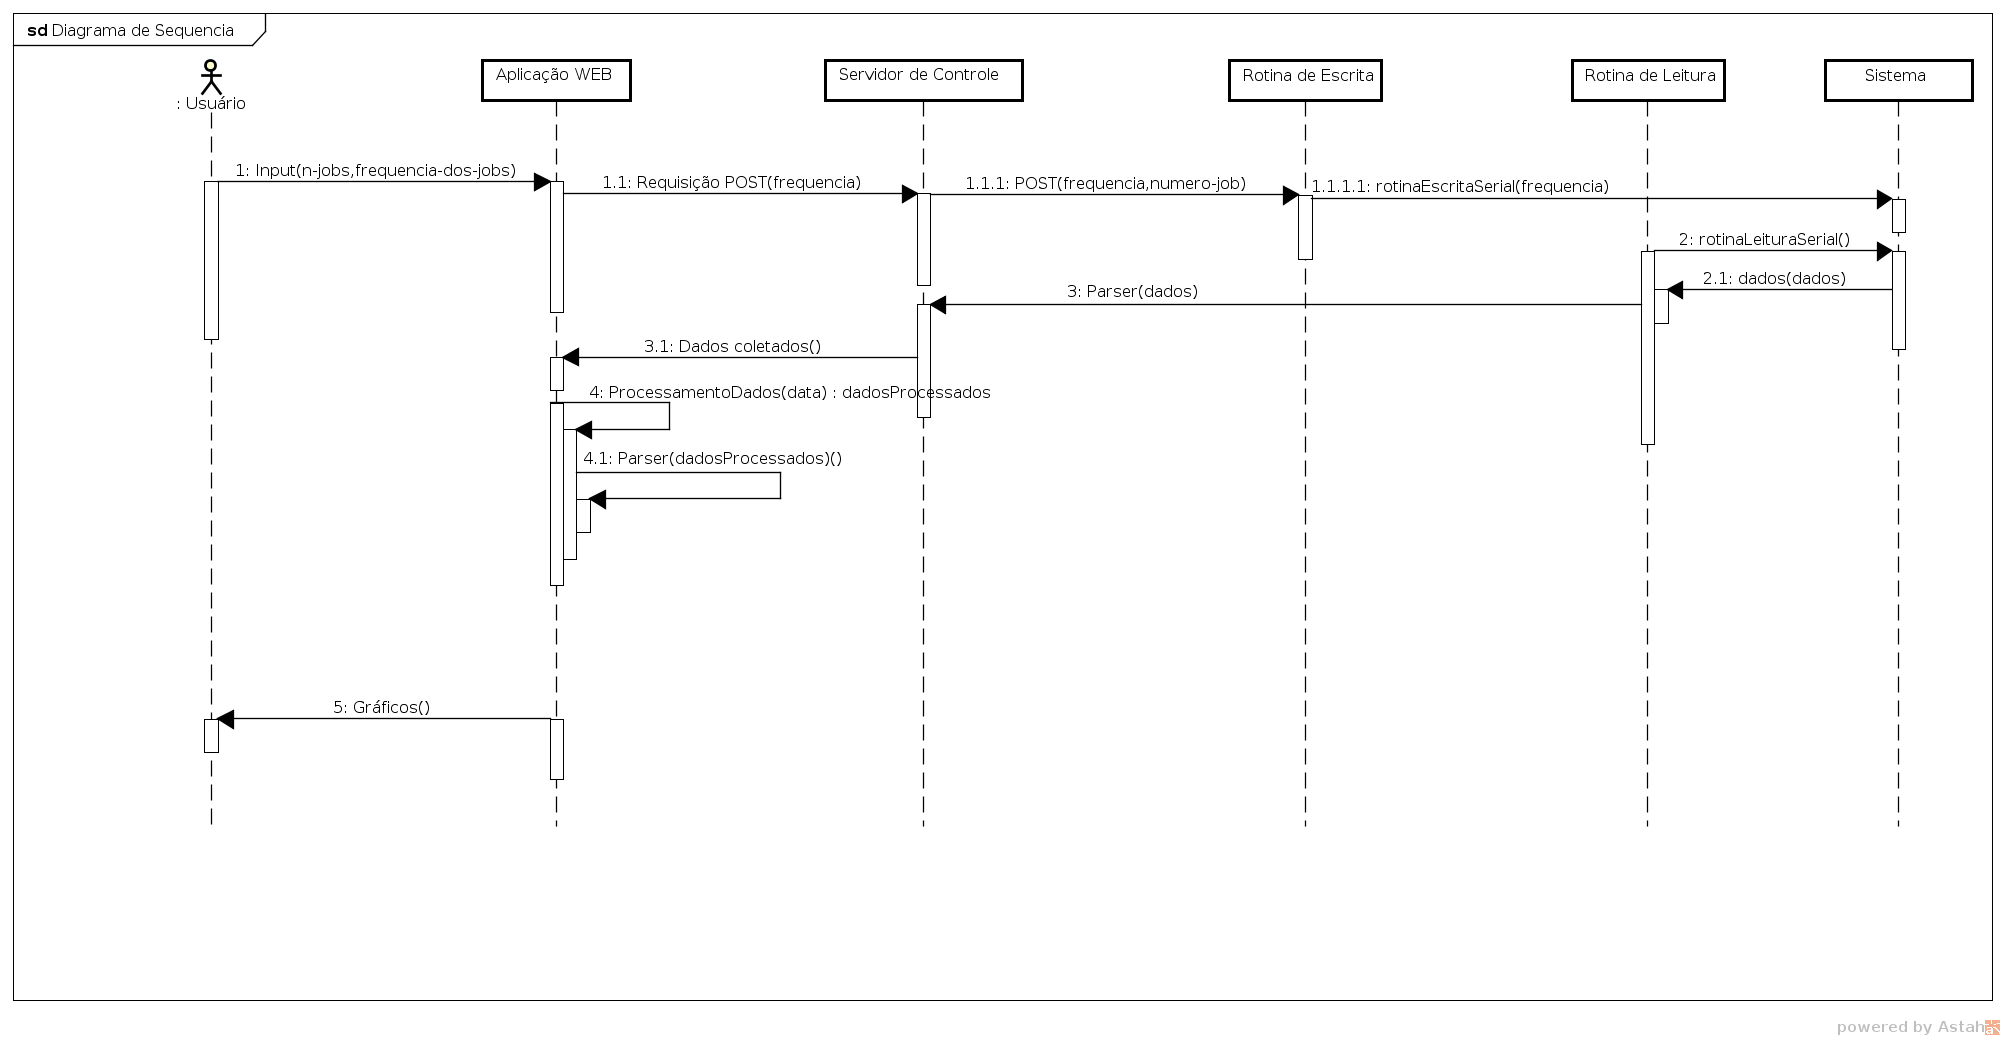
\includegraphics[keepaspectratio=true,scale=0.5,angle=90]{figuras/diagrama_sequencia.png}
\caption{Diagrama de sequência - Fonte: Autor}
\end{figure}
